% ==============================================================================
% Modelo para Especificação de Requisitos de Software
% Prof. Vítor E. Silva Souza - NEMO/UFES :: DI/UFES :: PPGI/UFES
%
% Baseado em abtex2-modelo-trabalho-academico.tex, v-1.9.2 laurocesar
% Copyright 2012-2014 by abnTeX2 group at http://abntex2.googlecode.com/ 
%
% This work may be distributed and/or modified under the conditions of the LaTeX 
% Project Public License, either version 1.3 of this license or (at your option) 
% any later version. The latest version of this license is in
% http://www.latex-project.org/lppl.txt.
%
% IMPORTANTE:
% Instruções encontram-se espalhadas pelo documento. Para facilitar sua leitura,
% tais instruções são precedidas por (*) -- utilize a função localizar do seu
% editor para passar por todas elas.
% ==============================================================================

% Usa o estilo abntex2, configurando detalhes de formatação e hifenização.
\documentclass[
12pt,				
oneside,		
a4paper,			
english,			% Idioma adicional para hifenização.
french,				% Idioma adicional para hifenização.
spanish,			% Idioma adicional para hifenização.
brazil				% O último idioma é o principal do documento.
]{abntex2}


%%% Importação de pacotes. %%%

% Conserta o erro "No room for a new \count". 
% O comando \reserveinserts deve ser comentado ou não, dependendo da versão do LaTeX.
\usepackage{etex}
%\reserveinserts{28}

% Usa a fonte Latin Modern.
\usepackage{lmodern}

% Seleção de códigos de fonte.
\usepackage[T1]{fontenc}

% Codificação do documento em Unicode.
\usepackage[utf8]{inputenc}

% Usado pela ficha catalográfica.
\usepackage{lastpage}

% Indenta o primeiro parágrafo de cada seção.
\usepackage{indentfirst}

% Controle das cores.
\usepackage[usenames,dvipsnames]{xcolor}

% Inclusão de gráficos.
\usepackage{graphicx}

% Melhor controle de leiaute de tabelas.
\usepackage{tabularx}
\usepackage{colortbl}
\usepackage{longtable}

% Adds PDF support to the environment landscape.
\usepackage{pdflscape}

% Inclusão de páginas em PDF diretamente no documento (para uso nos apêndices).
\usepackage{pdfpages}

% Para melhorias de justificação.
\usepackage{microtype}

% Citações padrão ABNT.
\usepackage[brazilian,hyperpageref]{backref}
\usepackage[alf]{abntex2cite}	
\renewcommand{\backrefpagesname}{Citado na(s) página(s):~}		% Usado sem a opção hyperpageref de backref.
\renewcommand{\backref}{}										% Texto padrão antes do número das páginas.
\renewcommand*{\backrefalt}[4]{									% Define os textos da citação.
	\ifcase #1
	Nenhuma citação no texto.
	\or
	Citado na página #2.
	\else
	Citado #1 vezes nas páginas #2.
	\fi}

% \rm is deprecated and should not be used in a LaTeX2e document
% http://tex.stackexchange.com/questions/151897/always-textrm-never-rm-a-counterexample
\renewcommand{\rm}{\textrm}

% Inclusão de símbolos não padrão.
\usepackage{amssymb}
\usepackage{eurosym}

% Para utilizar \eqref para referenciar equações.
\usepackage{amsmath}

% Permite mostrar figuras muito largas em modo paisagem com \begin{sidewaysfigure} ao invés de \begin{figure}.
\usepackage{rotating}

% Permite customizar listas enumeradas/com marcadores.
\usepackage{enumitem}

% Permite inserir hiperlinks com \url{}.
\usepackage{bigfoot}
\usepackage{hyperref}

% Permite usar o comando \hl{} para evidenciar texto com fundo amarelo. Útil para chamar atenção a itens a fazer.
\usepackage{soulutf8}

% Colorinlistoftodos package: to insert colored comments so authors can collaborate on the content.
% (*) Indicar o nome do aluno e substituir o nome do professor se for o caso.
\usepackage[colorinlistoftodos, textwidth=20mm, textsize=footnotesize]{todonotes}
\newcommand{\aluno}[1]{\todo[author=\textbf{Aluno},color=green!30,caption={},inline]{#1}}
\newcommand{\vitor}[1]{\todo[author=\textbf{Vítor},color=red!30,caption={},inline]{#1}}

% Permite inserir espaço em branco condicional (incluído no texto final só se necessário) em macros.
\usepackage{xspace}

% Permite incluir listagens de código com o comando \lstinputlisting{}.
\usepackage{listings}
\usepackage{caption}
\DeclareCaptionFont{white}{\color{white}}
\DeclareCaptionFormat{listing}{\colorbox{gray}{\parbox{\textwidth}{#1#2#3}}}
\captionsetup[lstlisting]{format=listing,labelfont=white,textfont=white}
\renewcommand{\lstlistingname}{Listagem}
\definecolor{mygray}{rgb}{0.5,0.5,0.5}
\lstset{
	basicstyle=\scriptsize,
	breaklines=true,
	numbers=left,
	numbersep=5pt,
	numberstyle=\tiny\color{mygray}, 
	rulecolor=\color{black},
	showstringspaces=false,
	tabsize=2,
	inputencoding=utf8,
	extendedchars=true,
	literate=%
	{é}{{\'{e}}}1
	{è}{{\`{e}}}1
	{ê}{{\^{e}}}1
	{ë}{{\¨{e}}}1
	{É}{{\'{E}}}1
	{Ê}{{\^{E}}}1
	{û}{{\^{u}}}1
	{ù}{{\`{u}}}1
	{â}{{\^{a}}}1
	{à}{{\`{a}}}1
	{á}{{\'{a}}}1
	{ã}{{\~{a}}}1
	{Á}{{\'{A}}}1
	{Â}{{\^{A}}}1
	{Ã}{{\~{A}}}1
	{ç}{{\c{c}}}1
	{Ç}{{\c{C}}}1
	{õ}{{\~{o}}}1
	{ó}{{\'{o}}}1
	{ô}{{\^{o}}}1
	{Õ}{{\~{O}}}1
	{Ó}{{\'{O}}}1
	{Ô}{{\^{O}}}1
	{î}{{\^{i}}}1
	{Î}{{\^{I}}}1
	{í}{{\'{i}}}1
	{Í}{{\~{Í}}}1
}




%%% Definição de variáveis. %%%
% (*) Substituir os textos abaixo com as informações apropriadas.
\titulo{Nome do Projeto}
\autor{Nome do Aluno}
\local{Vitória, ES}
\data{\the\year}

\instituicao{
	Universidade Federal do Espírito Santo -- UFES
	\par
	Centro Tecnológico
	\par
	Departamento de Informática}
\newcommand{\subtitulo}{Documento de Requisitos de Sistema}
\newcommand{\versao}{1.0}

% Define a capa.
% (*) Incluir linhas no registro de alterações a cada nova versão.
\renewcommand{\imprimircapa}{%
	\begin{capa}%
		\center
		
		{\ABNTEXchapterfont\large\subtitulo{}}
		\vfill
		\begin{center}
			\ABNTEXchapterfont\bfseries\LARGE\imprimirtitulo
		\end{center}
		
		\vfill
		Registro de Alterações:
		\begin{table}[h]
			\centering
			\vspace{0.5cm}
			\begin{tabular}{|c|c|c|p{4.5cm}|} \hline \rowcolor[rgb]{0.8,0.8,0.8}
 				
 				Versão & Responsável & Data  & Alterações \\	\hline  
 				                            
				1.0  & \imprimirautor & dd/MM/yyyy & Versão Inicial  \\ \hline 
			 
			\end{tabular}
		\end{table}
		
		\vfill
		\large\imprimirlocal
		\linebreak
		\large\imprimirdata
		\vspace*{1cm}
	\end{capa}
}

% Macros específicas do trabalho.
% (*) Inclua aqui termos que são utilizados muitas vezes e que demandam formatação especial.
% Exemplo: Java com TM (trademark) em superscript.
% Use sempre \xspace para que o LaTeX inclua espaço em branco após a macro somente quando necessário.
\newcommand{\java}{Java\texttrademark\xspace}




%%% Configurações finais de aparência. %%%

% Altera o aspecto de algumas cores.
\definecolor{blue}{RGB}{41,5,195}
\definecolor{lightgray}{gray}{0.9}

% Informações do PDF.
\makeatletter
\hypersetup{
	pdftitle={\@title}, 
	pdfauthor={\@author},
	pdfsubject={\imprimirpreambulo},
	pdfcreator={LaTeX with abnTeX2},
	pdfkeywords={abnt}{latex}{abntex}{abntex2}{trabalho acadêmico}, 
	colorlinks=true,				% Colore os links (ao invés de usar caixas).
	linkcolor=blue,					% Cor dos links.
	citecolor=blue,					% Cor dos links na bibliografia.
	filecolor=magenta,				% Cor dos links de arquivo.
	urlcolor=blue,					% Cor das URLs.
	bookmarksdepth=4
}
\makeatother

% Espaçamentos entre linhas e parágrafos.
\setlength{\parindent}{1.3cm}
\setlength{\parskip}{0.2cm}



%%% Páginas iniciais do documento: capa, folha de rosto, ficha, resumo, tabelas, etc. %%%

% Compila o índice.
\makeindex

% Inicia o documento.
\begin{document}

% Retira espaço extra obsoleto entre as frases.
\frenchspacing

% Inclui o brasão da UFES.
\begin{figure}[h]
	\centering
	
\includegraphics[scale=0.055]{brasao.jpg}
	\label{ppts3}
\end{figure} 

% Capa do trabalho.
\imprimircapa





%%% Início da parte de conteúdo do documento. %%%
% Marca o início dos elementos textuais.
\textual

% Inclusão dos capítulos.
% (*) Para facilitar a organização, os capítulos foram divididos em arquivo separados e colocados dentro da.
% pasta capitulos/. Caso o aluno prefira trabalhar com um só arquivo, basta substituir os comandos \include 
% pelos conteúdos dos arquivos que estão sendo incluídos, excluindo a pasta capitulos/ em seguida.

% ==============================================================================
% TCC - Nome do Aluno
% Capítulo 1 - Introdução
% ==============================================================================
\chapter{Introdução}
\label{sec-intro}

\hl{Texto.}

\hrulefill

Além do template pronto para uso, este documento inclui exemplos de uso de \latex que podem ser úteis para aqueles que possuem pouca experiência com a ferramenta. Quando for começar a escrever seu PG, apague todo o conteúdo abaixo da palavra ``Texto''.



%%% Início de seção. %%%
\section{Seções e subseções}
\label{sec-intro-secoes}

O documento é organizado em capítulos (\texttt{\textbackslash chapter\{\}}), seções (\texttt{\textbackslash section\{\}}), subseções (\texttt{\textbackslash subsection\{\}}), sub-subseções (\texttt{\textbackslash subsubsection\{\}}) e assim por diante. Atenção, porém, a não criar estruturas muito profundas (sub-sub-sub-...) pois o documento não fica bem estruturado.


%%% Início de seção. %%%
\subsection{Referências a seções}
\label{sec-intro-secoes-refs}

Cada parte do documento (capítulo, seção, etc.) deve possuir um rótulo logo abaixo de sua definição. Por exemplo, este capítulo é definido com \texttt{\textbackslash chapter\{Introdução\}} seguido por \texttt{\textbackslash label\{sec-intro\}}. Assim, podemos fazer referências cruzadas usando o comando \texttt{\textbackslash ref\{rótulo\}}: ``O Capítulo~\ref{sec-intro} começa com a Seção~\ref{sec-intro-secoes}, que é ainda subdividida nas subseções~\ref{sec-intro-secoes-refs} e~\ref{sec-intro-secoes-sobrerefs}.

Para melhor organização das partes do documento, sugere-se primeiro utilizar o prefixo \texttt{sec-} (para diferenciar de referências à figuras, tabelas, etc. quando usarmos o comando \texttt{\textbackslash ref\{\}}) e também representar a hierarquia das seções nos rótulos. Por exemplo, o Capítulo~\ref{sec-intro} tem rótulo \texttt{sec-intro}, sua Seção~\ref{sec-intro-secoes} tem rótulo \texttt{sec-intro-secoes} e a Subseção~\ref{sec-intro-secoes-refs} tem rótulo \texttt{sec-intro-secoes-refs}.



%%% Início de seção. %%%
\subsection{Sobre referências cruzadas}
\label{sec-intro-secoes-sobrerefs}

Nas próximas seções, veremos que é possível fazer referência cruzada não só a seções mas também a listagens de código, figuras, tabelas, etc. Em todos estes casos, quando nos referimos à Seção X, Listagem Y ou Figura Z, consideramos que estes são os nomes próprios destes elementos e, portanto, usa-se a primeira letra maiúscula. Isso pode ser visto na Subseção~\ref{sec-intro-secoes-refs}, acima. A exceção é quando nos referimos a vários elementos ao mesmo tempo, por exemplo: ``as subseções~\ref{sec-intro-secoes-refs} e~\ref{sec-intro-secoes-sobrerefs}''.

Por fim, ao usar o comando \texttt{\textbackslash ref\{\}}, sugere-se separá-lo da palavra que vem antes dele com um \textasciitilde\ ao invés de espaço. Por exemplo: \texttt{o capítulo\textasciitilde \textbackslash ref\{sec-intro\}}. Isso faz com que o \latex não quebre linha entre a palavra \texttt{capítulo} e o número do capítulo.




%%% Início de seção. %%%
\section{Citações bibliográficas}
\label{sec-intro-citacoes}

Este documento utiliza a ferramenta de gerenciamento de referências bibliográficas do \latex, chamada \emph{BibTeX}. O arquivo \texttt{bibliografia.bib}, referenciado no arquivo \latex principal deste documento, contém algumas referências bibliográficas de exemplo. Assim como capítulos, seções, etc., tais referências também possuem rótulos, especificados como primeiro parâmetro de cada entrada (ex.: \texttt{@incollection\{souza-et-al:iism08, ...\}}.

Sugere-se um padrão para rótulos de referências bibliográficas para que fique claro também no código \latex qual referência está sendo citada. Por exemplo, ao citar a referência \texttt{souza-et-al:sesas13}, sabemos que é um artigo escrito por \emph{Souza} e outros, publicado no \emph{SESAS} em \emph{2013} (geralmente a pessoa que citou sabe que publicação é SESAS e quem é Souza).

Para citar uma referência bibliográfica contida no arquivo \emph{BibTeX}, basta usar seu rótulo como parâmetro de um de dois comandos possíveis de citação:

\begin{itemize}
	\item O comando \texttt{\textbackslash cite\{\}} efetua uma citação tradicional, colocando o nome do(s) autor(es) e o ano entre parênteses. Por exemplo, \texttt{\textbackslash cite\{souza-et-al:iism08\}} é transformado em \cite{souza-et-al:iism08};
	
	\item O comando \texttt{\textbackslash citeonline\{\}} efetua uma citação integrada ao texto, colocando o nome do(s) autor(es) direto no texto e somente o ano entre parênteses. Por exemplo, ``de acordo com \texttt{\textbackslash citeonline\{souza-et-al:iism08\}}'' é transformado em: de acordo com \citeonline{souza-et-al:iism08};
\end{itemize}

Também é possível citar vários trabalhos de uma só vez, separando os rótulos das referências bibliográficas com uma vírgula dentro do comando apropriado. Por exemplo, \texttt{\textbackslash cite\{souza-et-al:sesas13,souza-et-al:csrd13\}} \cite{souza-et-al:sesas13,souza-et-al:csrd13}.

Os trabalhos citados são automaticamente incluídos na seção de referências bibliográficas, ao final do documento. Tudo é formatado automaticamente segundo padrões da ABNT.



%%% Início de seção. %%%
\section{Listagens de código}
\label{sec-intro-listagens}

O pacote \texttt{listings}, incluído neste template, permite a inclusão de listagens de código. Análogo ao já feito anteriormente, listagens possuem rótulos para que possam ser referenciadas e sugerimos uma regra de nomenclatura para tais rótulos: usar como prefixo o rótulo do capítulo, substituindo \texttt{sec-} por \texttt{lst-}.

A Listagem~\ref{lst-intro-exemplo}, por exemplo, possui o rótulo \texttt{lst-intro-exemplo} e representa o código que foi usado no próprio documento para exibir as listagens desta seção. Como podemos ver, a sugestão é que os arquivos de código sejam colocados dentro da pasta \texttt{codigos/} e tenham nome idêntico ao rótulo, colocando a extensão adequada ao tipo de código.

\lstinputlisting[label=lst-intro-exemplo, caption=Exemplo de código \latex para inclusão de listagens de código., float=htpb]{codigos/lst-intro-exemplo.tex}

A Listagem~\ref{lst-intro-outroexemplo} mostra um exemplo de listagem com especificação da linguagem utilizada no código. O pacote \texttt{listings} reconhece algumas linguagens\footnote{Veja a lista de linguagens suportadas em \url{http://en.wikibooks.org/wiki/LaTeX/Source\_Code\_Listings\#Supported_languages}.} e faz ``coloração'' de código (na verdade, usa \textbf{negrito} e não cores) de acordo com a linguagem. O parâmetro \texttt{float=htpb} incluído em ambos os exemplos impede que a listagem seja quebrada em diferentes páginas.

\lstinputlisting[label=lst-intro-outroexemplo, caption=Exemplo de código \java especificando linguagem utilizada., language=Java, float=htpb]{codigos/lst-intro-outroexemplo.java}



%%% Início de seção. %%%
\section{Figuras}
\label{sec-intro-figuras}

Figuras podem ser inseridas no documento usando o \emph{ambiente} \texttt{figure} (ou seja, \texttt{\textbackslash begin\{figure\}} e \texttt{\textbackslash end\{figure\}}) e o comando \texttt{\textbackslash includegraphics\{\}}. Existem alguns outros elementos e propriedades úteis de serem configuradas, resultando no código exibido na Listagem~\ref{lst-intro-figuras}.

\lstinputlisting[label=lst-intro-figuras, caption=Código \latex utilizado para inclusão das figuras na Seção~\ref{sec-intro-figuras}., float=htpb]{codigos/lst-intro-figuras.tex}

O comando \texttt{\textbackslash centering} centraliza a figura na página. A opção \texttt{width} do comando \texttt{\textbackslash includegraphics\{\}} determina o tamanho da figura e usa-se \texttt{\textbackslash textwidth} (opcionalmente multiplicado por um número) para se referir à largura da página.

O parâmetro do comando \texttt{\textbackslash includegraphics\{\}} indica onde a imagem pode ser encontrada. Foi criado o diretório \texttt{figuras/} para conter as figuras do documento, dando uma melhor organização aos arquivos. Ao abrir esta pasta, repare que as figuras possuem duas versões---uma em \texttt{.eps} e outra em \texttt{.pdf}---e que o comando \texttt{\textbackslash includegraphics\{\}} não especifica a extensão. Isso se dá porque o \latex possui um compilador para formato PostScript (\texttt{latex}) que espera as imagens em \texttt{.eps} e um compilador para PDF (\texttt{pdflatex}) que espera as imagens em \texttt{.pdf}. Dependendo do seu ambiente \latex, é possível apenas colocar as figuras em formatos mais comuns, como JPG ou PNG e ele incluir no PDF sem problemas. Vale a pena testar.

Por fim, o comando \texttt{\textbackslash caption\{\}} especifica a descrição da figura e \texttt{\textbackslash label\{\}}, como de costume, estabelece um rótulo para permitir referência cruzada de figuras. Note ainda que é utilizada a mesma estratégia de nomenclatura de rótulos usada nas listagens, porém utilizando o prefixo \texttt{fig-}.

As figuras~\ref{fig-intro-nemologo} e~\ref{fig-intro-exemplosideways} mostram o resultado do código da Listagem~\ref{lst-intro-figuras}. A Figura~\ref{fig-intro-exemplosideways}, em particular, utiliza o pacote \texttt{rotating} para mostrar figuras largas em modo paisagem. Basta usar o ambiente \texttt{sidewaysfigure} ao invés de \texttt{figure}.

\begin{figure}
	\centering
	
\includegraphics[width=.25\textwidth]{figuras/fig-intro-nemologo} 
	\caption{Exemplo de figura: logo do Nemo.}
	\label{fig-intro-nemologo}
\end{figure}

\begin{sidewaysfigure}
	\centering
	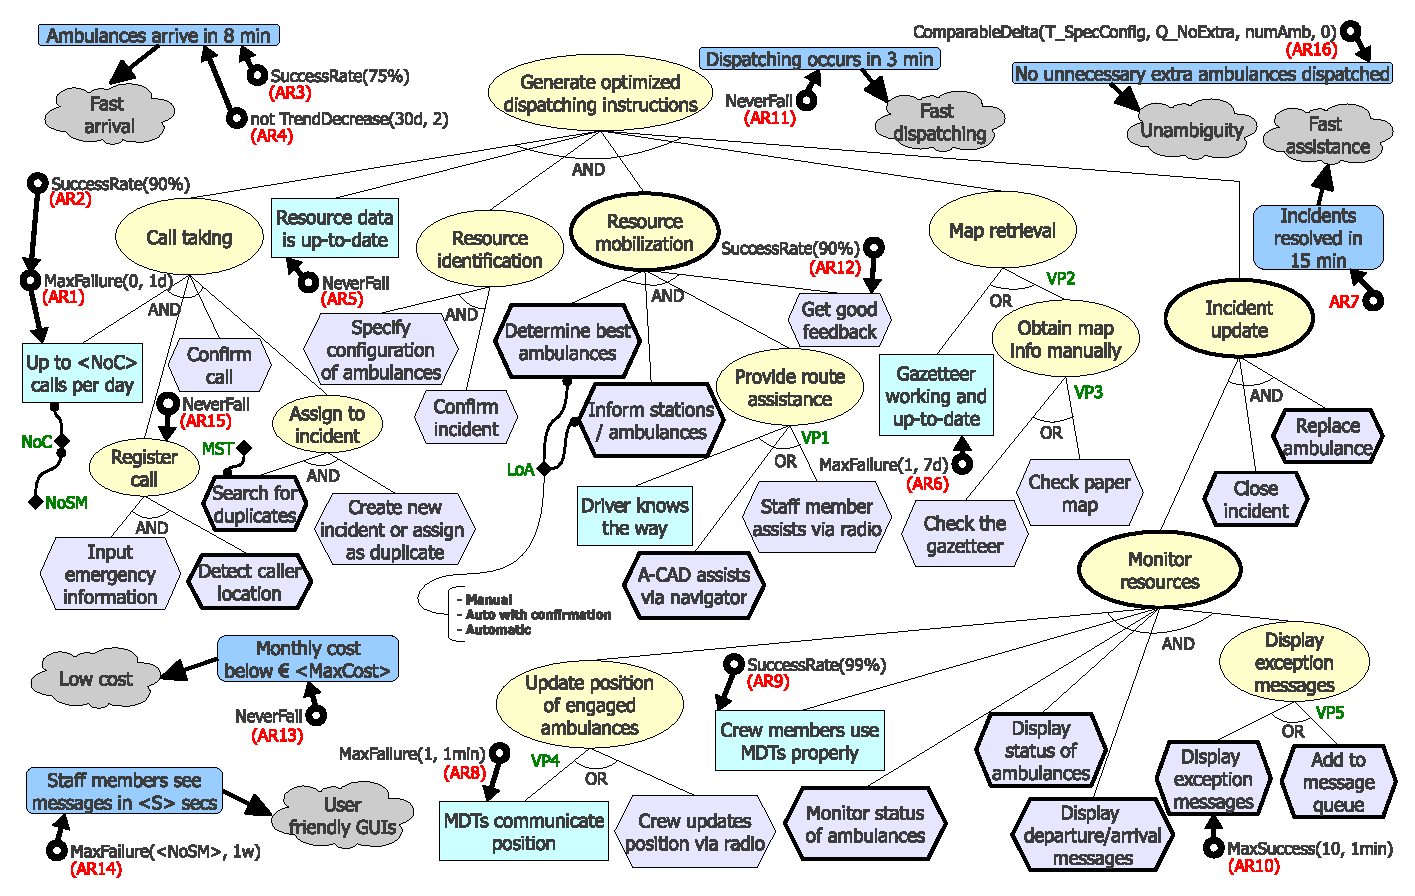
\includegraphics[width=\textwidth]{figuras/fig-intro-exemplosideways} 
	\caption{Exemplo de figura em modo paisagem: um modelo de objetivos~\cite{souza-mylopoulos:spe13}.}
	\label{fig-intro-exemplosideways}
\end{sidewaysfigure}



%%% Início de seção. %%%
\section{Tabelas}
\label{sec-intro-tabelas}

Tabelas são um ponto fraco do \latex. Elas são complicadas de fazer e, dependendo da complexidade da tabela (muitas células mescladas, por exemplo), vale a pena construi-las em outro programa (por exemplo, em seu editor de texto favorito) e inclui-las no documento como figuras. Mostramos, no entanto, alguns exemplos de tabela a seguir. O código utilizado para criar as tabelas encontra-se nas listagens~\ref{lst-intro-tabelas01}, \ref{lst-intro-tabelas02} e~\ref{lst-intro-tabelas03}.

\lstinputlisting[label=lst-intro-tabelas01, caption=Código \latex utilizado para inclusão das tabelas~\ref{tbl-intro-exemplo01} e~\ref{tbl-intro-exemplo02}., float=htpb]{codigos/lst-intro-tabelas01.tex}

\lstinputlisting[label=lst-intro-tabelas02, caption=Código \latex utilizado para inclusão da Tabela~\ref{tbl-intro-exemplo03}., float=htpb]{codigos/lst-intro-tabelas02.tex}

\lstinputlisting[label=lst-intro-tabelas03, caption=Código \latex utilizado para inclusão da Tabela~\ref{tbl-intro-exemplo04}., float=htpb]{codigos/lst-intro-tabelas03.tex}

Em particular, a Tabela~\ref{tbl-intro-exemplo04} utiliza um pacote chamado \texttt{tabularx}, que permite maior controle do layout das tabelas. Ao definir o ambiente \texttt{\textbackslash begin\{tabularx\}}, são definidos os tamanhos de cada coluna proporcional à largura ocupada pela tabela. Veja na Listagem~\ref{lst-intro-tabelas03} que as primeiras duas colunas não definem o atributo \texttt{\textbackslash hsize}, o que faz com que elas fiquem com o tamanho padrão de coluna, que é a largura da tabela dividida pelo número de colunas. Já a terceira coluna define \texttt{\textbackslash hsize=1.2\textbackslash hsize}, ou seja, esta coluna deve ser 20\% maior do que o tamanho padrão. Para isso, é preciso retirar de outras colunas, portanto a quarta e quinta colunas são definidas como 10\% menores (ou seja, \texttt{\textbackslash hsize=0.9\textbackslash hsize}).

% Exemplo de tabela 01:
\begin{table}
	\caption{Exemplo de tabela com diferentes alinhamentos de conteúdo.}
	\label{tbl-intro-exemplo01}
	\centering
	\begin{tabular}{ | c | l | r | p{40mm} |}\hline
		\textbf{Centralizado} & \textbf{Esquerda} & \textbf{Direita} & \textbf{Parágrafo}\\\hline
		C & L & R & Alinhamento de tipo parágrafo especifica largura da coluna e quebra o texto automaticamente.\\
		\hline
		Linha 2 & Linha 2 & Linha 2 & Linha 2\\
		\hline
	\end{tabular}
\end{table}

% Exemplo de tabela 02:
\begin{table}
	\caption{Exemplo que especifica largura de coluna e usa lista enumerada (adaptada de~\cite{souza-mylopoulos:spe13}).}
	\label{tbl-intro-exemplo02}
	\centering
	\renewcommand{\arraystretch}{1.2}
	\begin{small}
		\begin{tabular}{ | p{15mm} | p{77mm} | p{55mm} |}\hline
			\textbf{\textit{AwReq}} & \textbf{Adaptation strategies} & \textbf{Applicability conditions}\\\hline
			
			AR1 &
			\vspace{-2mm}\begin{enumerate}[topsep=0cm, partopsep=0cm, itemsep=0cm, parsep=0cm, leftmargin=0.5cm]
				\item \textit{Warning(``AS Management'')}
				\item \textit{Reconfigure($\varnothing$)}
			\end{enumerate}\vspace{-4mm} &
			\vspace{-2mm}\begin{enumerate}[topsep=0cm, partopsep=0cm, itemsep=0cm, parsep=0cm, leftmargin=0.5cm]
				\item Once per adaptation session;
				\item Always.
			\end{enumerate}\vspace{-4mm}
			\\\hline
			
			AR2 &
			\vspace{-2mm}\begin{enumerate}[topsep=0cm, partopsep=0cm, itemsep=0cm, parsep=0cm, leftmargin=0.5cm]
				\item \textit{Warning(``AS Management'')}
				\item \textit{Reconfigure($\varnothing$)}
			\end{enumerate}\vspace{-4mm} &
			\vspace{-2mm}\begin{enumerate}[topsep=0cm, partopsep=0cm, itemsep=0cm, parsep=0cm, leftmargin=0.5cm]
				\item Once per adaptation session;
				\item Always.
			\end{enumerate}\vspace{-4mm}
			\\\hline
		\end{tabular}
	\end{small}
\end{table}

% Exemplo de tabela 03:
\begin{table}
	\caption{Exemplo que mostra equações em duas colunas (adaptada de~\cite{souza-mylopoulos:spe13}).}
	\label{tbl-intro-exemplo03}
	\centering
	\vspace{1mm}
	\fbox{\begin{minipage}{.98\linewidth}
			\begin{minipage}{0.51\linewidth}
				\vspace{-4mm}
				\begin{eqnarray}
				\Delta \left( I_{AR1} / NoSM \right) \left[ 0, maxSM \right] > 0\\
				\Delta \left( I_{AR2} / NoSM \right) \left[ 0, maxSM \right] > 0\\
				\Delta \left( I_{AR3} / LoA \right) < 0\\
				\end{eqnarray}
				\vspace{-6mm}
			\end{minipage}
			\hspace{2mm}
			\vline 
			\begin{minipage}{0.41\linewidth}
				\vspace{-4mm}
				\begin{eqnarray}
				\Delta \left( I_{AR11} / VP2 \right) < 0\\
				\Delta \left( I_{AR12} / VP2 \right) > 0\\
				\Delta \left( I_{AR6} / VP3 \right) > 0\\
				\end{eqnarray}
				\vspace{-6mm}
			\end{minipage}
	\end{minipage}}
\end{table}

% Exemplo de tabela 04:
\begin{table}[h]
	\caption{Exemplo que utiliza o pacote \texttt{tabularx}, extraído de um artigo ainda não publicado.}
	\label{tbl-intro-exemplo04}
	\centering\tiny\def\tabularxcolumn#1{m{#1}}
	\begin{tabularx}{\columnwidth}{ >{\centering}X | >{\centering}X | >{\hsize=1.2\hsize\centering}X | >{\hsize=0.9\hsize\centering}X | >{\hsize=0.9\hsize\centering\arraybackslash}X }
		\hline
		\textbf{Applied Criteria} & \textbf{Analyzed Content} & \textbf{Initial\\Occurrences} & \textbf{Final Results} & \textbf{Reduction (\%)} \\
		\hline
		Duplicate Removal & Title, authors and year & 903 & 420 & 54,84\% \\ 
		\hline 
		IC and ECs & Title, abstract and keywords & 420 & 130 & 69,05\% \\ 
		\hline 
		IC and ECs & Full text & 130 & 117 & 10\% \\ 
		\hline 
		Final Results & -- & 903 & 117 & 87,04\% \\ 
		\hline 
	\end{tabularx}
\end{table}

\chapter{Descrição do Propósito do Sistema}
\label{sec-proposito}

\vitor{Utilizando 1 a 3 parágrafos, estabelecer o contexto que motiva o desenvolvimento do sistema em questão e descrever seu propósito.}



\chapter{Descrição do Minimundo}
\label{sec-minimundo}

\vitor{De forma mais detalhada (vários parágrafos, possivelmente dividir em subseções), descrever o minimundo do sistema, ou seja, o domínio no qual ele se encaixa, quais os problemas que pretende resolver, por meio de quais funcionalidades.}



% Escolher entre requisitos funcionais ou estórias de usuário.
%\chapter{Requisitos de Usuário}
\label{sec-requisitos}

\vitor{Listar os principais \textit{stakeholders} do projeto no parágrafo abaixo e preencher as tabelas de requisitos funcionais, não funcionais e regras de negócio, com atenção aos identificadores e \textit{labels}.}

Tomando por base o contexto do sistema descrito na Seção~\ref{sec-minimundo} e considerando como principais \textit{stakeholders} \hl{(listar aqui os principais stakeholders do projeto)}, foram identificados os seguintes requisitos de usuário e regras de negócio.



% Define contador e identificador para requisitos funcionais.
% Usar \RF\label{rf-nome-do-label} para cada requisito definido.
\newcounter{rfcount}
\renewcommand*\therfcount{RF-\arabic{rfcount}}
\newcommand*\RF{\refstepcounter{rfcount}\therfcount}
\setcounter{rfcount}{0}

% Tabela de requisitos funcionais.
\begin{longtable}{|c|p{9cm}|c|p{2.2cm}|}
	\caption{Requisitos Funcionais.}
	\label{tbl-requisitos-rfs} \\\hline 
	
	% Cabeçalho e repetição do mesmo em cada nova página. Manter como está.
	\rowcolor{lightgray}
	\textbf{ID} & \textbf{Descrição} & \textbf{Prioridade} & \textbf{Depende} \\\hline	
	\endfirsthead
	\hline
	\rowcolor{lightgray}
	\textbf{ID} & \textbf{Descrição} & \textbf{Prioridade} & \textbf{Depende} \\\hline	
	\endhead
	
	% Especificar os requisitos abaixo, substituindo os exemplos.
	\RF\label{rf-exemplo-01} &  O sistema deve ...  & Alta & \\\hline
	
	\RF\label{rf-exemplo-02} &  O sistema deve ...  & Alta & \ref{rf-exemplo-01} \\\hline

	\RF\label{rf-exemplo-03} &  O sistema deve ...  & Alta & \ref{rf-exemplo-01}, \ref{rf-exemplo-02} \\\hline
\end{longtable}



% Define contador e identificador para requisitos não funcionais.
% Usar \RNF\label{rnf-nome-do-label} para cada requisito definido.
\newcounter{rnfcount}
\renewcommand*\thernfcount{RNF-\arabic{rnfcount}}
\newcommand*\RNF{\refstepcounter{rnfcount}\thernfcount}
\setcounter{rnfcount}{0}

% Tabela de requisitos não funcionais.
\begin{longtable}{|c|p{5.3cm}|c|c|c|}
	\caption{Requisitos Não Funcionais.}
	\label{tbl-requisitos-rnfs} \\\hline 
	
	% Cabeçalho e repetição do mesmo em cada nova página. Manter como está.
	\rowcolor{lightgray}
	\textbf{ID} & \textbf{Descrição} & \textbf{Categoria} & \textbf{Escopo} & \textbf{Prioridade} \\\hline		
	\endfirsthead
	\hline
	\rowcolor{lightgray}
	\textbf{ID} & \textbf{Descrição} & \textbf{Categoria} & \textbf{Escopo} & \textbf{Prioridade} \\\hline		
	\endhead
	
	% Especificar os requisitos abaixo, substituindo os exemplos.
	\RNF\label{rnf-exemplo-01} & Descrição sucinta. & Característica & Funcionalidade & Baixa \\\hline 	

	\RNF\label{rnf-exemplo-02} & Descrição sucinta. & de & ou & Média \\\hline 	

	\RNF\label{rnf-exemplo-03} & Descrição sucinta. & qualidade & Sistema & ou Alta \\\hline
\end{longtable}



% Define contador e identificador para regras de negócio.
% Usar \RN\label{rn-nome-do-label} para cada regra definida.
\newcounter{rncount}
\renewcommand*\therncount{RN-\arabic{rncount}}
\newcommand*\RN{\refstepcounter{rncount}\therncount}
\setcounter{rncount}{0}

% Tabela de regras de negócio.
\begin{longtable}{|c|p{9cm}|c|p{2.2cm}|}
	\caption{Regras de Negócio.}
	\label{tbl-requisitos-rns} \\\hline 
	
	% Cabeçalho e repetição do mesmo em cada nova página. Manter como está.
	\rowcolor{lightgray}
	\textbf{ID} & \textbf{Descrição} & \textbf{Prioridade} & \textbf{Depende} \\\hline	
	\endfirsthead
	\hline
	\rowcolor{lightgray}
	\textbf{ID} & \textbf{Descrição} & \textbf{Prioridade} & \textbf{Depende} \\\hline	
	\endhead
	
	% Especificar as regras abaixo, substituindo os exemplos.
	\RN\label{rn-exemplo-01} & Descrição sucinta. & Baixa & \ref{rf-exemplo-01} \\\hline

	\RN\label{rn-exemplo-02} & Descrição sucinta. & Média & \ref{rf-exemplo-01}, \ref{rf-exemplo-02} \\\hline

	\RN\label{rn-exemplo-03} & Descrição sucinta. & ou Alta & \ref{rf-exemplo-03} \\\hline
\end{longtable}

\chapter{Requisitos de Usuário}
\label{sec-requisitos}

\vitor{Está sendo utilizado o \textit{template} que lista as estórias de usuário. Existe também um \textit{template} para os requisitos funcionais, basta modificar o arquivo \texttt{ch4-} que está sendo incluído no documento principal.}

\vitor{Listar os principais \textit{stakeholders} do projeto no parágrafo abaixo e preencher as tabelas de estórias de usuário, requisitos não-funcionais e regras de negócio, com atenção aos identificadores e \textit{labels}.}

Tomando por base o contexto do sistema descrito na Seção~\ref{sec-minimundo} e considerando como principais \textit{stakeholders} \hl{(listar aqui os principais stakeholders do projeto)}, foram identificadas estórias de usuário, requisitos não funcionais e regras de negócio.

As estórias de usuário são apresentadas na Tabela~\ref{tbl-requisitos-uss}, os requisitos não-funcionais na Tabela~\ref{tbl-requisitos-rnfs} e as regras de negócio globais (aquelas que não são caracterizadas como critérios de aceitação de estórias de usuário específica) na Tabela~\ref{tbl-requisitos-rns}. As tabelas são apresentadas nas páginas a seguir, em formato paisagem, para melhor visualização.

% Mostra as tabelas em formato paisagem.
\begin{landscape}

% Define contador e identificador para estórias de usuário.
% Usar \US\label{rf-nome-do-label} para cada requisito definido.
\newcounter{uscount}
\renewcommand*\theuscount{US-\arabic{uscount}}
\newcommand*\US{\refstepcounter{uscount}\theuscount}
\setcounter{uscount}{0}

% Tabela de requisitos funcionais.
\begin{longtable}{|c|p{8cm}|p{9.7cm}|c|p{2.2cm}|}
	\caption{Estórias de Usuário.}
	\label{tbl-requisitos-uss} \\\hline 
	
	% Cabeçalho e repetição do mesmo em cada nova página. Manter como está.
	\rowcolor{lightgray}
	\textbf{ID} & \textbf{Descrição} & \textbf{Critérios de Aceitação} & \textbf{Prioridade} & \textbf{Depende} \\\hline	
	\endfirsthead
	\hline
	\rowcolor{lightgray}
	\textbf{ID} & \textbf{Descrição} & \textbf{Critérios de Aceitação} & \textbf{Prioridade} & \textbf{Depende} \\\hline	
	\endhead
	
	% Especificar as estórias de usuário abaixo, substituindo os exemplos.
	\US\label{us-exemplo-01} & 
		\hl{Genérico: } Como \hl{ator}, quero \hl{função}, para \hl{finalidade}. &
		\parbox{9.7cm}{
		\begin{enumerate}[leftmargin=15mm,label=-- CA\arabic*:]\itemsep-2mm
			\item Critério de aceitação 1;
			\item Critério de aceitação 2;
			\item Critério de aceitação N.
		\end{enumerate}
		} & Baixa & \\\hline
	
	\US\label{us-exemplo-02} & 
		\hl{Cadastro/CRUD: } Como \hl{ator}, quero cadastrar \hl{objeto}, para \hl{finalidade}. &
		\parbox{9.7cm}{
		\begin{enumerate}[leftmargin=15mm,label=-- CA\arabic*:]\itemsep-2mm
			\item Para cadastrar um \hl{objeto} devem ser informados \hl{campos};
			\item Um \hl{objeto} não pode ter as seguintes informações alteradas: \hl{campos};
			\item A consulta pode ser feita por \hl{campos};
			\item \hl{Objetos} relacionados a \hl{outros objetos} não podem ser excluídos;
			\item Alterações ou exclusões devem ser comunicadas e/ou deve ser requerida confirmação.
		\end{enumerate}
		} & Média & \ref{us-exemplo-01} \\\hline

	\US\label{us-exemplo-03} & 
		\hl{Consulta: } Como \hl{ator}, quero consultar \hl{informações}, para \hl{finalidade}. &
		\parbox{9.7cm}{
		\begin{enumerate}[leftmargin=15mm,label=-- CA\arabic*:]\itemsep-2mm
			\item Para realizar a consulta, o usuário deve informar como parâmetros: \hl{parâmetros};
			\item Devem ser apresentadas as seguintes informações para o usuário: \hl{campos}.
		\end{enumerate}
		} & ou Alta & \ref{us-exemplo-01}, \ref{us-exemplo-02} \\\hline
\end{longtable}



% Define contador e identificador para requisitos não funcionais.
% Usar \RNF\label{rnf-nome-do-label} para cada requisito definido.
\newcounter{rnfcount}
\renewcommand*\thernfcount{RNF-\arabic{rnfcount}}
\newcommand*\RNF{\refstepcounter{rnfcount}\thernfcount}
\setcounter{rnfcount}{0}

% Tabela de requisitos não funcionais.
\begin{longtable}{|c|p{14.3cm}|c|c|c|}
	\caption{Requisitos Não Funcionais.}
	\label{tbl-requisitos-rnfs} \\\hline 
	
	% Cabeçalho e repetição do mesmo em cada nova página. Manter como está.
	\rowcolor{lightgray}
	\textbf{ID} & \textbf{Descrição} & \textbf{Categoria} & \textbf{Escopo} & \textbf{Prioridade} \\\hline		
	\endfirsthead
	\hline
	\rowcolor{lightgray}
	\textbf{ID} & \textbf{Descrição} & \textbf{Categoria} & \textbf{Escopo} & \textbf{Prioridade} \\\hline		
	\endhead
	
	% Especificar os requisitos abaixo, substituindo os exemplos.
	\RNF\label{rnf-exemplo-01} & Descrição sucinta. & Característica & Funcionalidade & Baixa \\\hline 	

	\RNF\label{rnf-exemplo-02} & Descrição sucinta. & de & ou & Média \\\hline 	

	\RNF\label{rnf-exemplo-03} & Descrição sucinta. & qualidade & Sistema & ou Alta \\\hline
\end{longtable}



% Define contador e identificador para regras de negócio.
% Usar \RN\label{rn-nome-do-label} para cada regra definida.
\newcounter{rncount}
\renewcommand*\therncount{RN-\arabic{rncount}}
\newcommand*\RN{\refstepcounter{rncount}\therncount}
\setcounter{rncount}{0}

% Tabela de regras de negócio.
\begin{longtable}{|c|p{18cm}|c|p{2.2cm}|}
	\caption{Regras de Negócio.}
	\label{tbl-requisitos-rns} \\\hline 
	
	% Cabeçalho e repetição do mesmo em cada nova página. Manter como está.
	\rowcolor{lightgray}
	\textbf{ID} & \textbf{Descrição} & \textbf{Prioridade} & \textbf{Depende} \\\hline	
	\endfirsthead
	\hline
	\rowcolor{lightgray}
	\textbf{ID} & \textbf{Descrição} & \textbf{Prioridade} & \textbf{Depende} \\\hline	
	\endhead
	
	% Especificar as regras abaixo, substituindo os exemplos.
	\RN\label{rn-exemplo-01} & Descrição sucinta. & Baixa & \ref{us-exemplo-01} \\\hline

	\RN\label{rn-exemplo-02} & \hl{Devem ser incluídas apenas regras de negócio globais.} & Média & \ref{us-exemplo-01}, \ref{us-exemplo-02} \\\hline

	\RN\label{rn-exemplo-03} & \hl{Regras de negócio associadas a uma estória de usuário específica devem constar como critério de aceitação da referida estória.} & ou Alta & \ref{us-exemplo-03} \\\hline
\end{longtable}

% Fim do formato paisagem.
\end{landscape}


\chapter{ Identificação de Subsistemas}
\label{sec-subsistemas}

Tal projeto foi dividido em 4 subsistemas a fim de facilitar o desenvolvimento de funcionalidades que são, de certa forma, isoladas, originando assim os subsistemas Auth, Log, Classroom e Board.
A Figura~\ref{figura-subsistema} mostra os subsistemas identificados no contexto do presente projeto e suas interdependências, enquanto a Tabela~\ref{tabela-subsistema} apresenta breve descrição de cada um deles.


\begin{figure}[h]
	\centering
	\includegraphics[width=\textwidth]{figuras/subsistemas.png}
	\caption{Diagrama de Pacotes e os Subsistemas Identificados.}
	\label{figura-subsistema}
\end{figure} 

\begin{table}[h]
	\centering	
	\vspace{0.5cm}
	\caption{ Subsistemas}
	\label{tabela-subsistema}
	\begin{tabular}{|p{3cm}|p{12cm}|}  \hline \rowcolor[rgb]{0.8,0.8,0.8}
		
		Subsistema & Descrição \\\hline 
		
		Classroom & Subsistema contendo as funcionalidades relacionadas diretamente às turmas.  \\\hline
		
		Board & Envolve todas as funcionalidades relativas ao gerenciamento dos itens do board. \\\hline
		
		Board Interactions & Corresponde a todas as interações que os usuários podem realizar com os itens do board, como submeter tarefas ou realizar provas. \\\hline
		
		Feedback & Permite a avaliação de atividades e a visualização das notas do aluno em uma turma. \\\hline
		
		Discussions & Subsistema contendo as funcionalidades relativas ao fórum de discussão, às notícias e às \textit{Live Questions}. \\\hline
		
		Logs & Este sistema consiste na visualização de logs gerados a partir das atividades dos usuários do sistema. \\\hline  
		
	\end{tabular}	
\end{table}


\chapter{Modelo de Casos de Uso}
\label{sec-caso-de-uso}

\newcounter{uccount}                                      \renewcommand*\theuccount{UC-\arabic{uccount}}
\newcommand*\UC{\refstepcounter{uccount}\theuccount}      \setcounter{uccount}{0}

O modelo de casos de uso corresponde a uma tentativa de descrever a relação das funcionalidades do sistema com cada um de seus atores. Os atores identificados no contexto deste projeto estão descritos na Tabela~\ref{tabela-atores}.

\begin{table}[H]
	\centering \vspace{0.5cm} \caption{ Atores}
	\begin{tabular}{|p{3cm}|p{12cm}|} \hline \rowcolor[rgb]{0.8,0.8,0.8}
		Ator & Descrição \\\hline                              
		Visitante & Qualquer pessoa que acesse o sistema e não tenha realizado o \textit{login}. \\\hline                              
		Administrador & Usuário que realizou o \textit{login} e pode gerenciar todo o sistema. \\\hline                              
		Membro & Usuário que realizou o \textit{login} no sistema mas que não possui permissões para configurá-lo. \\\hline	                              
		Aluno & Corresponde a um Membro vinculado a alguma turma com permissões de aluno, como enviar tarefas e consultas notas. \\\hline	                              
		Professor & Corresponde a um Membro vinculado a alguma turma com permissões de professor, como criar itens do \textit{board} e configurar as informações da turma. \\\hline			 
	\end{tabular}
	\label{tabela-atores}	
\end{table}

A seguir, são apresentados os diagramas de casos de uso e descrições associadas, organizados por subsistema.
	
\section{Subsistema Classroom}

A Figura~\ref{figura-caso-de-uso-classroom} apresenta o diagrama de casos de uso do subsistema Classroom.

\begin{figure}[h!]
	\centering
	\includegraphics[width=\textwidth]{figuras/casos-de-uso-classroom.png}
	\caption{Diagrama de Casos de Uso do subsistema Classroom.}
	\label{figura-caso-de-uso-classroom}
\end{figure}

Com exceção do \ref{uc-definir-configuracoes}, todos os outros casos de uso abaixo mencionados geram um \textit{Log} indicando o usuário que realizou a ação, qual ação foi tomada e o momento em que isso aconteceu. Além disso, cada \textit{Log} fica associado a uma determinada categoria. Por exemplo, o \ref{uc-enviar-mensagens} pertenceria à categoria "Envio de mensagens".


A seguir, são apresentadas as descrições de cada um dos casos de uso identificados. Os casos de uso cadastrais de baixa complexidade, envolvendo inclusão, alteração, consulta e exclusão, são descritos na Tabela~\ref{tabela-classroom-cadastrais}.


\begin{table}[H]
	\centering  \vspace{0.5cm} 	\footnotesize 
	\caption{Casos de Uso Cadastrais}
	\begin{tabular}{|c|c|c|p{6cm}|p{1.5cm}|p{2cm}|} \hline  \rowcolor[rgb]{0.8,0.8,0.8}
		
		Id & Nome  &  Ações  &  Observações & Requisitos   & Classes  \\ 	\hline \hline	
		
		{}  &  {}  &  I   & Informar: título e senha de acesso. Opcionalmente, também é possível escolher professores da turma caso estes já estejam cadastrados no sistema. &   {}   & {}    \\\cline{3-4}
		{}  &  {}  &  A   &  {}   &   {}   &  {}  \\ \cline{3-4}
		{}  &  {}  &  C  &   {}   &   {}  &   {}    \\\cline{3-4}
		\multirow{-4}{*}{\UC\label{uc-gerenciar-turmas}}   &  \multirow{-4}{*}{\parbox{2cm}{Gerenciar turmas}}   &    E    &    A exclusão de uma turma deve acarretar na exclusão de todos os itens de \textit{board} e suas interações (como submissões de tarefa e respostas de provas).   &  \multirow{-4}{1.5cm}{\ref{rf-criar-turma}}  & \multirow{-4}{2cm}{Classroom}  \\ \hline 
		
		{}  &  {}  &  I   &  Informar: título, descrição, data e tipo (Evento ou Aula). &   {}   & {}    \\\cline{3-4}
		{}  &  {}  &  A   &  {}   &   {}   &  {}  \\ \cline{3-4}
		{}  &  {}  &  C  &   {}   &   {}  &   {}    \\\cline{3-4}
		\multirow{-5}{*}{\UC\label{uc-gerenciar-calendario}}   &  \multirow{-5}{*}{\parbox{2cm}{Gerenciar eventos no calendário}}   &    E    &   {}   &  \multirow{-5}{1.5cm}{\ref{rf-gerenciamento-calendario}}  & \multirow{-5}{2cm}{Classroom, Event, Class}  \\ \hline 
		
		
	\end{tabular}
	\label{tabela-classroom-cadastrais}
\end{table}

Os casos de uso de consulta mais abrangente que as consultas a um único objeto, mas ainda de baixa complexidade, tais como consultas que combinam informações de vários objetos envolvendo filtros, estão descritos na Tabela~\ref{tabela-khoeus-consulta}.

\begin{table}[H]
	\centering  \vspace{0.5cm} 	\footnotesize 
	\caption{Casos de Uso de Consulta}
	\begin{tabular}{|c|p{2.3cm}|p{6.8cm}|c|p{1.8cm}|} \hline  \rowcolor[rgb]{0.8,0.8,0.8}
		
		Id & Nome   &  Observações & Requisitos   & Classes  \\ 	\hline	
		
		
		\UC\label{uc-consultar-presencas} & Consultar suas presenças & Os alunos de uma turma terão acesso ao seu quadro de presenças contendo a lista de aulas do curso em que estão inscritos e se estiveram presentes (ou não) nas aulas que já ocorreram.  &    \ref{rf-consultar-presenca}        & User, Classroom, Class e Presence\\ \hline
		
		
		\UC\label{uc-consultar-calendario} & Consultar calendário & Os alunos de uma turma terão acesso ao calendário contendo as aulas e eventos registrados para aquela turma. Para cada um, exibe-se o nome, a descrição (caso tenha) e a data em que acontecerá. &   \ref{rf-acessar-calendario}        & User, Classroom, Class e Event	\\ \hline
		
	\end{tabular}
	\label{tabela-khoeus-consulta}
\end{table}

\clearpage
\begin{flushright}    \textbf{Descrição de Caso de Uso}   \end{flushright}         
\noindent \textbf{Projeto:} \imprimirtitulo  \\
\textbf{Identificador do Caso de Uso:} \UC\label{uc-definir-configuracoes} \\
\textbf{Caso de Uso:} Definir configurações do sistema \\
\noindent \textbf{Descrição Sucinta:} Este caso de uso permite que o usuário altere as principais configurações do sistema, acessíveis apenas para administradores.\\

\begin{table}[H]
	\centering \vspace{0.5cm} \footnotesize
	\caption{Fluxos de Eventos Normais}
	\begin{tabular}{|p{2.3cm}|p{2.5cm}|p{10cm}|} \hline  \rowcolor[rgb]{0.8,0.8,0.8}
		
		Nome do Fluxo & Precondição & Descrição  \\ \hline		
		
		Definir configurações & O usuário  deverá estar logado e& 1. O administrador poderá alterar todas as configurações do sistema listadas no \ref{rf-configuracoes}  \\
		{} & ser um administrador & 2. Ao finalizar, o sistema salva todas essas alterações de forma genérica, armazenando o nome da configuração bem como seu respectivo valor.\\ \hline
		
		
	\end{tabular}
\end{table}

\noindent  \textbf{Requisitos Relacionados:} \ref{rf-configuracoes}       \\ \textbf{Classes Relacionadas:} User, Configuration.

\newpage
\clearpage
\begin{flushright}    \textbf{Descrição de Caso de Uso}   \end{flushright}         
\noindent \textbf{Projeto:} \imprimirtitulo  \\
\textbf{Identificador do Caso de Uso:} \UC\label{uc-ingressar-turma} \\
\textbf{Caso de Uso:} Ingressar em uma turma \\
\noindent \textbf{Descrição Sucinta:} Este caso de uso permite que um usuário se vincule a uma turma por meio de uma chave de inscrição.\\

\begin{table}[H]
	\centering \vspace{0.5cm} \footnotesize
	\caption{Fluxos de Eventos Normais}
	\begin{tabular}{|p{2.3cm}|p{2.5cm}|p{10cm}|} \hline  \rowcolor[rgb]{0.8,0.8,0.8}
		
		Nome do Fluxo & Precondição & Descrição  \\ \hline		
		
		Ingressar em uma turma & O usuário  deverá estar logado & 1. O usuário deverá escolher a turma que deseja ingressar e informar a senha de acesso fornecida por um  dos professores.  \\
		{} & {} & 2. O sistema vincula aquele usuário àquela turma em uma \textit{role} de aluno, garantindo que este possa acessá-la a qualquer momento.\\ \hline	
	\end{tabular}
\end{table}

\begin{table}[H]
	\centering \vspace{0.5cm} \footnotesize
	\caption{Fluxos de Eventos Variantes}
	\begin{tabular}{|p{2.3cm}|p{1.8cm}|p{10.7cm}|} \hline  \rowcolor[rgb]{0.8,0.8,0.8}
		
		Nome do Fluxo & Variante & Descrição  \\ \hline		
		
		Chave incorreta & O usuário digitou a chave de inscrição incorreta & 1.  O sistema informa que a chave de inscrição está errada e solicita que o usuário tente novamente.  \\ \hline 
		
	\end{tabular}
\end{table}


\noindent  \textbf{Requisitos Relacionados:} \ref{rf-inscricao}       \\ \textbf{Classes Relacionadas:} User, Classroom, Subscription.

\newpage
\clearpage
\begin{flushright}    \textbf{Descrição de Caso de Uso}   \end{flushright}         
\noindent \textbf{Projeto:} \imprimirtitulo  \\
\textbf{Identificador do Caso de Uso:} \UC\label{uc-lancar-presenca} \\
\textbf{Caso de Uso:} Lançar presença \\
\noindent \textbf{Descrição Sucinta:} Este caso de uso permite que o professor lance a presença dos alunos de sua turma para cada uma das aulas cadastradas no calendário.\\

\begin{table}[H]
	\centering \vspace{0.5cm} \footnotesize
	\caption{Fluxos de Eventos Normais}
	\begin{tabular}{|p{2.3cm}|p{2.5cm}|p{10cm}|} \hline  \rowcolor[rgb]{0.8,0.8,0.8}
		
		Nome do Fluxo & Precondição & Descrição  \\ \hline		
		
		Lançar presença & O usuário  deverá estar logado e& 1. O usuário deverá informar em uma tabela aluno x aula se o aluno esteve presente (ou não) na aula em questão.  \\
		{} & ser um professor da turma correspondente & 2. O sistema salva uma presença para cada um dos alunos que compareceram à(s) aula(s).\\ \hline
		
		
	\end{tabular}
\end{table}


\noindent  \textbf{Requisitos Relacionados:} \ref{rf-lancar-presenca}       \\ \textbf{Classes Relacionadas:} User, Classroom, Class, Presence.

\newpage
\clearpage
\begin{flushright}    \textbf{Descrição de Caso de Uso}   \end{flushright}         
\noindent \textbf{Projeto:} \imprimirtitulo  \\
\textbf{Identificador do Caso de Uso:} \UC\label{uc-definir-roles} \\
\textbf{Caso de Uso:} Definir \textit{roles} de usuários nas turmas \\
\noindent \textbf{Descrição Sucinta:} Este caso de uso permite que um administrador possa conceder a \textit{role} de professor ou de usuário a um determinado aluno.\\

\begin{table}[H]
	\centering \vspace{0.5cm} \footnotesize
	\caption{Fluxos de Eventos Normais}
	\begin{tabular}{|p{2.3cm}|p{2.5cm}|p{10cm}|} \hline  \rowcolor[rgb]{0.8,0.8,0.8}
		
		Nome do Fluxo & Precondição & Descrição  \\ \hline		
		
		Definir \textit{roles} & O usuário  deverá estar logado e ser um & 1. Em uma lista de todos os usuários inscritos naquela turma, o administrador poderá escolher qual será a \textit{role} associada àquele usuário naquela turma.  \\
		{} &  administrador do sistema  & 2.  O sistema salva a nova \textit{role} do(s) usuário(s), garantindo novas permissões para aqueles que foram alterados.\\ \hline
		
		
	\end{tabular}
\end{table}


\noindent  \textbf{Requisitos Relacionados:} \ref{rf-gerenciamento-usuario-turma}, \ref{rn-roles}       \\ \textbf{Classes Relacionadas:} User, Classroom, Subscription.

\newpage
\clearpage
\begin{flushright}    \textbf{Descrição de Caso de Uso}   \end{flushright}         
\noindent \textbf{Projeto:} \imprimirtitulo  \\
\textbf{Identificador do Caso de Uso:} \UC\label{uc-configurar-turma} \\
\textbf{Caso de Uso:} Configurar turma \\
\noindent \textbf{Descrição Sucinta:} Este caso de uso permite que o professor altere as configurações de uma turma.\\

\begin{table}[H]
	\centering \vspace{0.5cm} \footnotesize
	\caption{Fluxos de Eventos Normais}
	\begin{tabular}{|p{2.3cm}|p{2.5cm}|p{10cm}|} \hline  \rowcolor[rgb]{0.8,0.8,0.8}
		
		Nome do Fluxo & Precondição & Descrição  \\ \hline		
		
		Configurar turma & O usuário  deverá estar logado e& 1. O usuário poderá alterar todas as configurações de turma listadas no \ref{rf-gerenciamento-turma}  \\
		{} & ser um professor da turma correspondente & 2.  Ao finalizar, o sistema salva todas essas alterações.\\ \hline
	\end{tabular}
\end{table}


\noindent  \textbf{Requisitos Relacionados:} \ref{rf-gerenciamento-turma}, \ref{rn-peso}       \\ \textbf{Classes Relacionadas:} User, Classroom.

\newpage
\clearpage
\begin{flushright}    \textbf{Descrição de Caso de Uso}   \end{flushright}         
\noindent \textbf{Projeto:} \imprimirtitulo  \\
\textbf{Identificador do Caso de Uso:} \UC\label{uc-enviar-mensagens} \\
\textbf{Caso de Uso:} Enviar mensagens \\
\noindent \textbf{Descrição Sucinta:} Este caso de uso permite que usuários de uma mesma turma troquem mensagens entre si.\\

\begin{table}[H]
	\centering \vspace{0.5cm} \footnotesize
	\caption{Fluxos de Eventos Normais}
	\begin{tabular}{|p{2.3cm}|p{2.5cm}|p{10cm}|} \hline  \rowcolor[rgb]{0.8,0.8,0.8}
		
		Nome do Fluxo & Precondição & Descrição  \\ \hline		
		
		Enviar mensagens & O usuário  deverá estar logado e& 1. O usuário deverá escolher para quem deseja enviar a mensagem e preencher o campo com o texto desejado. \\
		{} & estar inscrito na turma correspondente & 2. O sistema armazena a mensagem enviada e envia um e-mail para o(s) destinatário(s) informando-o(s) sobre a nova mensagem. \\ \hline
		
		
	\end{tabular}
\end{table}

\noindent  \textbf{Requisitos Relacionados:} \ref{rf-enviar-mensagem}, \ref{rn-mensagem}       \\ \textbf{Classes Relacionadas:} User, Message.

\newpage

\section{Subsistema Board}

A Figura~\ref{figura-caso-de-uso-board} apresenta o diagrama de casos de uso do subsistema Board.

\begin{figure}[h!]
	\centering
	\includegraphics[width=\textwidth]{figuras/casos-de-uso-board.png}
	\caption{Diagrama de Casos de Uso do Subsistema Board.}
	\label{figura-caso-de-uso-board}
\end{figure}

Todos os casos de uso mencionados geram um \textit{Log} indicando o usuário que realizou a ação, qual ação foi tomada e o momento em que isso aconteceu. Além disso, cada \textit{Log} fica associado a uma determinada categoria. Por exemplo, o \ref{uc-gerenciar-arquivos} pertenceria à categoria ``Gerenciamento de arquivos''.

A seguir, são apresentadas as descrições de cada um dos casos de uso identificados. Os casos de uso cadastrais de baixa complexidade, envolvendo inclusão, alteração, consulta e exclusão, são descritos na Tabela~\ref{tabela-board-cadastrais}.


\begin{longtable}{|c|c|c|p{6.3cm}|p{1.2cm}|p{2cm}|}
	\caption{Casos de Uso Cadastrais}\\
	 \hline  \rowcolor[rgb]{0.8,0.8,0.8}
		
		Id & Nome  &  Ações  &  Observações & Requisitos   & Classes  \\ 	\hline \hline
		\endhead
		\hline
		\endlastfoot
		
		{}  &  {}  &  I   & Informar: título e, opcionalmente, descrição. No momento da criação da seção, deve-se escolher a posição do \textit{board} em que esta será inserida. &   {}   & {}    \\\cline{3-4}
		{}  &  {}  &  A   &  {}   &   {}   &  {}  \\ \cline{3-4}
		{}  &  {}  &  C  &   {}   &   {}  &   {}    \\\cline{3-4}
		\multirow{-4}{*}{\UC\label{uc-gerenciar-secoes}}   &  \multirow{-4}{*}{\parbox{2cm}{Gerenciar seções do \textit{board}}}   &    E    &    A exclusão de uma seção deverá excluir todos os itens de \textit{board} associados a ela.   &  \multirow{-4}{1.5cm}{ \ref{rf-adicionar-secao}}  & \multirow{-4}{2cm}{User, Classroom e Section}  \\ \hline 
		
		{}  &  {}  &  I   &  A seção à qual o arquivo estará vinculado será escolhida antes de sua criação. Informar título, descrição e realizar o upload do arquivo desejado. No momento da criação do arquivo, deve-se escolher a posição da seção em que esta será inserido.&   {}   & {}    \\\cline{3-4}
		{}  &  {}  &  A   &  {}   &   {}   &  {}  \\ \cline{3-4}
		{}  &  {}  &  C  &   {}   &   {}  &   {}    \\\cline{3-4}
		\multirow{-7}{*}{\UC\label{uc-gerenciar-arquivos}}   &  \multirow{-7}{*}{\parbox{2cm}{Gerenciar arquivos do \textit{board}}}   &    E    &    {}   &  \multirow{-7}{1.5cm}{ \ref{rf-adicionar-arquivo} \ref{rn-item-secao}}  & \multirow{-7}{2cm}{User, Classroom, Section e File}  \\ \hline 
		
		{}  &  {}  &  I   &  A seção à qual o link estará vinculado será escolhida antes de sua criação. Informar título, descrição e o link desejado. No momento da criação do link, deve-se escolher a posição da seção em que esta será inserido. &   {}   & {}    \\\cline{3-4}
		{}  &  {}  &  A   &  {}   &   {}   &  {}  \\ \cline{3-4}
		{}  &  {}  &  C  &   {}   &   {}  &   {}    \\\cline{3-4}
		\multirow{-6}{*}{\UC\label{uc-gerenciar-links}}   &  \multirow{-6}{*}{\parbox{2cm}{Gerenciar links do \textit{board}}}   &    E    &    {}   &  \multirow{-6}{1.5cm}{ \ref{rf-adicionar-link}, \ref{rn-item-secao}}  & \multirow{-6}{2cm}{User, Classroom, Section e Link}  \\ \hline 
		
		{}  &  {}  &  I   &  A seção à qual o questionário estará vinculado será escolhida antes de sua criação. Informar título, descrição, data de início, data de encerramento, as perguntas do questionário e suas respectivas alternativas. No momento da criação do questionário, deve-se escolher a posição da seção em que esta será inserido. &   {}   & {}    \\\cline{3-4}
		{}  &  {}  &  A   &  {}   &   {}   &  {}  \\ \cline{3-4}
		{}  &  {}  &  C  &   {}   &   {}  &   {}    \\\cline{3-4}
		\multirow{-8}{*}{\UC\label{uc-gerenciar-questionarios}}   &  \multirow{-8}{*}{\parbox{2cm}{Gerenciar questionários do \textit{board}}}   &    E    &    A exclusão de um questionário deverá resultar na exclusão de todas as respostas que já foram enviadas.   &  \multirow{-8}{1.5cm}{ \ref{rf-adicionar-questionario}, \ref{rn-item-secao}}  & \multirow{-8}{2cm}{User, Classroom, Section, Survey, SurveyQuestion e SurveyAnswer}  \\ \hline 
		
		{}  &  {}  &  I   &  A seção à qual a prova estará vinculada será escolhida antes de sua criação. Informar título, descrição, data de início, data de encerramento, as questões da prova, seus valores (nota máxima) e seus respectivos tipos (discursiva ou objetiva). No caso de questões objetivas, o professor deverá informar suas alternativas e qual delas é a correta em cada questão. No momento da criação da prova, deve-se escolher a posição da seção em que esta será inserida.&   {}   & {}    \\\cline{3-4}
		{}  &  {}  &  A   &  {}   &   {}   &  {}  \\ \cline{3-4}
		{}  &  {}  &  C  &   {}   &   {}  &   {}    \\\cline{3-4}
		\multirow{-10}{*}{\UC\label{uc-gerenciar-provas}}   &  \multirow{-10}{*}{\parbox{2cm}{Gerenciar provas do \textit{board}}}   &    E    &    A exclusão de uma prova deverá resultar na exclusão de todas as resoluções que já foram enviadas.   &  \multirow{-10}{1.5cm}{ \ref{rf-adicionar-prova}, \ref{rn-item-secao}}  & \multirow{-10}{2cm}{User, Classroom, Section, Test, TestQuestion e Text Alternative}  \\ \hline 
		
		{}  &  {}  &  I   &  A seção à qual a tarefa estará vinculada será escolhida antes de sua criação. Informar título, descrição, data de início, data de encerramento e o tipo de tarefa. No caso de tarefas do tipo arquivo, deve-se informar o número máximo de arquivos que poderão ser submetidos. No momento da criação da tarefa, deve-se escolher a posição da seção em que esta será inserida.&   {}   & {}    \\\cline{3-4}
		{}  &  {}  &  A   &  {}   &   {}   &  {}  \\ \cline{3-4}
		{}  &  {}  &  C  &   {}   &   {}  &   {}    \\\cline{3-4}
		\multirow{-8}{*}{\UC\label{uc-gerenciar-tarefas}}   &  \multirow{-8}{*}{\parbox{2cm}{Gerenciar tarefas do \textit{board}}}   &    E    &    A exclusão de uma tarefa deverá resultar na exclusão de todas as submissões que já foram feitas e de seus respectivos feedbacks.   &  \multirow{-8}{1.5cm}{ \ref{rf-adicionar-tarefa}, \ref{rn-item-secao}}  & \multirow{-8}{2cm}{User, Classroom, Section e Assignment}  \\ \hline 
		
		
		{}  &  {}  &  I   &  A seção à qual a atividade externa estará vinculada será escolhida antes de sua criação. Informar título e descrição. No momento da criação da atividade externa, deve-se escolher a posição da seção em que esta será inserida. &   {}   & {}    \\\cline{3-4}
		{}  &  {}  &  A   &  {}   &   {}   &  {}  \\ \cline{3-4}
		{}  &  {}  &  C  &   {}   &   {}  &   {}    \\\cline{3-4}
		\multirow{-7}{*}{\UC\label{uc-gerenciar-atividadesexternas}}   &  \multirow{-7}{*}{\parbox{2cm}{Gerenciar atividades externas do \textit{board}}}   &    E    &    A exclusão de uma atividade externa deverá resultar na exclusão de todas as atividades associadas a ela.   &  \multirow{-7}{1.5cm}{ \ref{rf-adicionar-atividadeexterna}, \ref{rn-item-secao}}  & \multirow{-7}{2cm}{User, Classroom, Section, External Activity} 
		
	\label{tabela-board-cadastrais}
\end{longtable}

\section{Subsistema Board Interactions}

A Figura~\ref{figura-caso-de-uso-board-interactions} apresenta o diagrama de casos de uso do subsistema Board Interactions.

\begin{figure}[h!]
	\centering
	\includegraphics[width=\textwidth]{figuras/casos-de-uso-board-interactions.png}
	\caption{Diagrama de Casos de Uso do Subsistema Board Interactions.}
	\label{figura-caso-de-uso-board-interactions}
\end{figure}

Todos os casos de uso mencionados geram um \textit{Log} indicando o usuário que realizou a ação, qual ação foi tomada e o momento em que isso aconteceu. Além disso, cada \textit{Log} fica associado a uma determinada categoria. Por exemplo, o \ref{uc-submeter-tarefa} pertenceria à categoria ``Submissão de tarefa''.

Para os casos de uso \ref{uc-responder-questionario}, \ref{uc-resolver-prova} e \ref{uc-submeter-tarefa}, a classe correspondente deve ser vinculada ao usuário que interagiu com ela. Por exemplo, no caso de uso \ref{uc-submeter-tarefa}, a classe Submission deve estar associada ao usuário que submeter aquela tarefa.

A seguir, são apresentadas as descrições de cada um dos casos de uso identificados. 


\clearpage
\begin{flushright}    \textbf{Descrição de Caso de Uso}   \end{flushright}         
\noindent \textbf{Projeto:} \imprimirtitulo  \\
\textbf{Identificador do Caso de Uso:} \UC\label{uc-download-arquivo} \\
\textbf{Caso de Uso:} Fazer download de arquivo \\
\noindent \textbf{Descrição Sucinta:} Este caso de uso permite que o usuário realize o download de um arquivo adicionado no \textit{board} da turma.\\

\begin{table}[H]
	\centering \vspace{0.5cm} \footnotesize
	\caption{Fluxos de Eventos Normais}
	\begin{tabular}{|p{2.3cm}|p{2.5cm}|p{10cm}|} \hline  \rowcolor[rgb]{0.8,0.8,0.8}
		
		Nome do Fluxo & Precondição & Descrição  \\ \hline		
		
		Fazer download & O usuário deverá estar logado e & 1. O usuário escolhe o item do \textit{board} de sua turma correspondente ao arquivo.  \\
		{}    & inscrito na turma correspondente & 2.  O download é iniciado pelo sistema.\\ \hline 
	\end{tabular}
\end{table}


\noindent  \textbf{Requisitos Relacionados:} \ref{rf-acessar-arquivo}       \\ \textbf{Classes Relacionadas:} User, Classroom e File.

\newpage
\clearpage
\begin{flushright}    \textbf{Descrição de Caso de Uso}   \end{flushright}         
\noindent \textbf{Projeto:} \imprimirtitulo  \\
\textbf{Identificador do Caso de Uso:} \UC\label{uc-acessar-link} \\
\textbf{Caso de Uso:} Acessar um link \\
\noindent \textbf{Descrição Sucinta:} Este caso de uso permite que o usuário acesse um link adicionado no \textit{board} da turma.\\

\begin{table}[H]
	\centering \vspace{0.5cm} \footnotesize
	\caption{Fluxos de Eventos Normais}
	\begin{tabular}{|p{2.3cm}|p{2.5cm}|p{10cm}|} \hline  \rowcolor[rgb]{0.8,0.8,0.8}
		
		Nome do Fluxo & Precondição & Descrição  \\ \hline		
		
		Acessar link & O usuário deverá estar logado e & 1. O usuário escolhe o item do \textit{board} de sua turma correspondente ao link.  \\
		{}    & inscrito na turma correspondente& 2. O navegador acessará a URL quando o usuário escolher o item do \textit{board} correspondente ao link.\\ \hline 
		
		
	\end{tabular}
\end{table}

\noindent  \textbf{Requisitos Relacionados:} \ref{rf-acessar-link}       \\ \textbf{Classes Relacionadas:} User, Classroom e Link.

\newpage
\clearpage
\begin{flushright}    \textbf{Descrição de Caso de Uso}   \end{flushright}         
\noindent \textbf{Projeto:} \imprimirtitulo  \\
\textbf{Identificador do Caso de Uso:} \UC\label{uc-responder-questionario} \\
\textbf{Caso de Uso:} Responder a um questionário \\
\noindent \textbf{Descrição Sucinta:} Este caso de uso permite que um aluno responda a um questionário em sua turma.\\

\begin{table}[H]
	\centering \vspace{0.5cm} \footnotesize
	\caption{Fluxos de Eventos Normais}
	\begin{tabular}{|p{2.3cm}|p{2.5cm}|p{10cm}|} \hline  \rowcolor[rgb]{0.8,0.8,0.8}
		
		Nome do Fluxo & Precondição & Descrição  \\ \hline		
		
		Responder questionário & O usuário deverá estar logado & 1. O usuário escolhe o item do \textit{board} de sua turma correspondente ao questionário que deseja responder.  \\
		{}    &  e inscrito na turma  & 2. O usuário deverá responder a todas as perguntas obrigatórias e submeter o questionário. \\
		{}    & correspondente & 3. O sistema armazena todas as respostas para aquele questionário.\\ \hline 
		
		Visualizar resultado de questionário & O usuário deverá estar logado & 1. O usuário escolhe o item do \textit{board} de sua turma correspondente ao questionário.  \\
		{}    &  e inscrito na turma correspondente  & 2. O usuário poderá visualizar o resultado do questionário. \\ \hline 
		
		
	\end{tabular}
\end{table}

\begin{table}[H]
	\centering \vspace{0.5cm} \footnotesize
	\caption{Fluxos de Eventos Variantes}
	\begin{tabular}{|p{2.3cm}|p{2.5cm}|p{10.0cm}|} \hline  \rowcolor[rgb]{0.8,0.8,0.8}
		
		Nome do Fluxo & Variante & Descrição  \\ \hline		
		
		Data limite atingida & O usuário tenta acessar um questionário em uma data posterior à limite & 1. Passada a data limite, o sistema avisa que o período para responder ao questionário já terminou.  \\ \hline 
		
	\end{tabular}
\end{table}

\noindent  \textbf{Requisitos Relacionados:} \ref{rf-acessar-questionario}, \ref{rn-submeter}       \\ \textbf{Classes Relacionadas:} User, Classroom, Survey, SurveyQuestion, SurveyAnswer e SurveyResponse.

\newpage
\clearpage
\begin{flushright}    \textbf{Descrição de Caso de Uso}   \end{flushright}         
\noindent \textbf{Projeto:} \imprimirtitulo  \\
\textbf{Identificador do Caso de Uso:} \UC\label{uc-resolver-prova} \\
\textbf{Caso de Uso:} Resolver uma prova \\
\noindent \textbf{Descrição Sucinta:} Este caso de uso permite que o usuário resolva as questões de uma prova, sendo elas discursivas ou objetivas.\\

\begin{table}[H]
	\centering \vspace{0.5cm} \footnotesize
	\caption{Fluxos de Eventos Normais}
	\begin{tabular}{|p{2.3cm}|p{2.5cm}|p{10cm}|} \hline  \rowcolor[rgb]{0.8,0.8,0.8}
		
		Nome do Fluxo & Precondição & Descrição  \\ \hline		
		
		Resolver  prova & O usuário  deverá estar logado e& 1. O usuário escolhe o item do \textit{board} de sua turma correspondente à prova desejada.  \\
		{}    &  inscrito na turma  & 2. O usuário deverá responder às perguntas objetivas e discursivas e submeter a prova.\\
		{}    &  correspondente & 3. O sistema armazena as respostas do aluno.\\ \hline
		
		
	\end{tabular}
\end{table}


\begin{table}[H]
	\centering \vspace{0.5cm} \footnotesize
	\caption{Fluxos de Eventos Variantes}
	\begin{tabular}{|p{2.3cm}|p{2.5cm}|p{10.0cm}|} \hline  \rowcolor[rgb]{0.8,0.8,0.8}
		
		Nome do Fluxo & Variante & Descrição  \\ \hline		
		
		Data limite atingida & O usuário tenta resolver uma prova em uma data posterior à limite & 1. Passada a data limite, o sistema exibe apenas a nota de cada questão e seu feedback.  \\ \hline 
		
	\end{tabular}
\end{table}


\noindent  \textbf{Requisitos Relacionados:} \ref{rf-acessar-prova}, \ref{rn-submeter}       \\ \textbf{Classes Relacionadas:} User, Classroom, Test, TestQuestion, TestAlternative, Test TextResponse e Test AlternativeResponse.

\newpage	
\clearpage
\begin{flushright}    \textbf{Descrição de Caso de Uso}   \end{flushright}         
\noindent \textbf{Projeto:} \imprimirtitulo  \\
\textbf{Identificador do Caso de Uso:} \UC\label{uc-submeter-tarefa} \\
\textbf{Caso de Uso:} Submeter uma tarefa \\
\noindent \textbf{Descrição Sucinta:} Este caso de uso permite que o usuário submeta uma tarefa do tipo especificado pelo professor no momento de sua criação.\\

\begin{table}[H]
	\centering \vspace{0.5cm} \footnotesize
	\caption{Fluxos de Eventos Normais}
	\begin{tabular}{|p{2.3cm}|p{2.5cm}|p{10cm}|} \hline  \rowcolor[rgb]{0.8,0.8,0.8}
		
		Nome do Fluxo & Precondição & Descrição  \\ \hline		
		
		Submeter tarefa & O usuário deverá estar logado e & 1. O usuário escolhe o item do \textit{board} de sua turma correspondente à tarefa desejada.  \\
		{}    &  inscrito na turma correspondente & 2. O usuário deverá submeter a tarefa da seguinte forma: caso a tarefa seja do tipo Texto ou Código, ele deverá preencher o campo com o texto/código correspondente. Caso a tarefa seja do tipo Arquivo, o usuário deverá fazer upload do(s) arquivo(s) correspondente(s). Caso a tarefa seja do tipo Código, o usuário deverá selecionar qual a linguagem de programação foi utilizada.\\
		{}    & {} & 3. O sistema armazena as informações da tarefa enviada. Caso esta seja do tipo Código, cada linha é armazenada separadamente. \\ \hline
		
		
	\end{tabular}
\end{table}

\begin{table}[H]
	\centering \vspace{0.5cm} \footnotesize
	\caption{Fluxos de Eventos Variantes}
	\begin{tabular}{|p{2.3cm}|p{2.5cm}|p{10cm}|} \hline  \rowcolor[rgb]{0.8,0.8,0.8}
		
		Nome do Fluxo & Variante & Descrição  \\ \hline		
		
		Data limite atingida & O usuário tenta submeter uma tarefa em uma data posterior à limite & 1. Passada a data limite, o sistema exibe apenas a nota da tarefa e seu feedback.  \\ \hline 
		
		Número de arquivos superior ao permitido & O usuário tenta submeter uma tarefa do tipo Arquivo fazendo upload de mais arquivos que o permitido & 1. O sistema informa o número máximo de arquivos que o usuário pode submeter.  \\ \hline 
		
	\end{tabular}
\end{table}


\noindent  \textbf{Requisitos Relacionados:} \ref{rf-acessar-tarefa}, \ref{rn-limite-arquivos}, \ref{rn-submeter}       \\ \textbf{Classes Relacionadas:} User, Classroom, Assignment, TextSubmission, CodeSubmission e FileSubmission.

\newpage


\section{Subsistema Feedback}

A Figura~\ref{figura-caso-de-uso-feedback} apresenta o diagrama de casos de uso do subsistema Feedback.

\begin{figure}[h!]
	\centering
	\includegraphics[width=\textwidth]{figuras/casos-de-uso-feedback.png}
	\caption{Diagrama de Casos de Uso do Subsistema Feedback.}
	\label{figura-caso-de-uso-feedback}
\end{figure}

Todos os casos de uso mencionados geram um \textit{Log} indicando o usuário que realizou a ação, qual ação foi tomada e o momento em que isso aconteceu. Além disso, cada \textit{Log} fica associado a uma determinada categoria. Por exemplo, o \ref{uc-consultar-notas} pertenceria à categoria ``Consulta de notas''.

A seguir, são apresentadas as descrições de cada um dos casos de uso identificados. Os casos de uso de consulta mais abrangente que as consultas a um único objeto, mas ainda de baixa complexidade, tais como consultas que combinam informações de vários objetos envolvendo filtros, estão descritos na Tabela~\ref{tabela-feedback-consulta}.

\begin{table}[H]
	\centering  \vspace{0.5cm} 	\footnotesize 
	\caption{Casos de Uso de Consulta}
	\begin{tabular}{|c|p{2cm}|p{5.7cm}|c|p{3.2cm}|} \hline  \rowcolor[rgb]{0.8,0.8,0.8}
		
		Id & Nome   &  Observações & Requisitos   & Classes  \\ 	\hline	
		
	
		\UC\label{uc-visualizar-resultado-prova} & Visualizar resultado da prova & O resultado de uma prova fica disponível para ser visualizado na tela de detalhamento da prova correspondente. Para cada prova, espera-se ver a resposta dada para cada questão, a nota atribuída a cada questão e o feedback dado pelo professor. &   \ref{rf-consultar-nota-prova}        & User, Classroom, Test, TestQuestion, TestAlternative, Test TextResponse e Test AlternativeResponse\\ \hline
		\UC\label{uc-visualizar-feedback-tarefa} & Visualizar feedback de tarefa & O resultado de uma tarefa fica disponível para ser visualizado na tela de detalhamento da tarefa correspondente. Para cada tarefa, espera-se ver a submissão feita (seja ela texto, arquivo ou código), a nota atribuída à tarefa e o feedback dado pelo professor.   &    \ref{rf-consultar-nota-tarefa}        & User, Classroom, Assignment, Submission, Text Submission, File Submission, Code Submission, Code Line, Code Line Feedback e Text Feedback\\ \hline
		\UC\label{uc-visualizar-nota-externa} & Visualizar nota de atividade externa & A nota de uma atividade externa fica disponível para ser visualizada na tela de detalhamento da atividade correspondente. Para cada atividade externa, espera-se ver a nota atribuída a ela e o feedback dado pelo professor. &   \ref{rf-consultar-nota-atividadeexterna}        & User, Classroom, External Activity e Activity\\ \hline
		\UC\label{uc-consultar-notas} & Consultar suas notas & Os alunos de uma turma terão acesso ao seu livro de notas. Para cada prova, tarefa e atividade externa realizada ao longo do curso, espera-se ver a nota atribuída a ela. Além disso, deve ser possível também consultar a média parcial no curso. &    \ref{rf-consultar-notas}        & User, Classroom, Grade Category, Assignment, Submission, Test,  Test Question, Test Alternative, Test TextResponse, Test AlternativeResponse, ExternalActivity e Activity	\\ \hline
		
		
	\end{tabular}
	\label{tabela-feedback-consulta}
\end{table}


\clearpage
\begin{flushright}    \textbf{Descrição de Caso de Uso}   \end{flushright}         
\noindent \textbf{Projeto:} \imprimirtitulo  \\
\textbf{Identificador do Caso de Uso:} \UC\label{uc-download-lote} \\
\textbf{Caso de Uso:} Fazer download em lote das submissões de uma tarefa ou prova \\
\noindent \textbf{Descrição Sucinta:} Este caso de uso permite que o professor efetue o download de todas as submissões de uma tarefa ou das respostas de uma prova simultaneamente.\\

\begin{table}[H]
	\centering \vspace{0.5cm} \footnotesize
	\caption{Fluxos de Eventos Normais}
	\begin{tabular}{|p{2.3cm}|p{2.5cm}|p{10cm}|} \hline  \rowcolor[rgb]{0.8,0.8,0.8}
		
		Nome do Fluxo & Precondição & Descrição  \\ \hline		
		
		Download em lote & O usuário deverá estar logado e & 1. O professor escolhe o item do \textit{board} de sua turma correspondente à tarefa/prova desejada.  \\
		{} &  ser professor na turma correspondente & 2. Ao clicar sobre o botão correspondente, dar-se-á início ao download de um arquivo compactado contendo todas as provas/tarefas submetidas.\\ \hline
		
		
	\end{tabular}
\end{table}


\noindent  \textbf{Requisitos Relacionados:} \ref{rf-download-lote}       \\ \textbf{Classes Relacionadas:} User, Classroom, Test, TestQuestion, TestAnswer, Assignment, TextSubmission, CodeSubmission e FileSubmission.

\newpage
\clearpage
\begin{flushright}    \textbf{Descrição de Caso de Uso}   \end{flushright}         
\noindent \textbf{Projeto:} \imprimirtitulo  \\
\textbf{Identificador do Caso de Uso:} \UC\label{uc-avaliar-individualmente} \\
\textbf{Caso de Uso:} Avaliar tarefas, provas ou atividades externas \\
\noindent \textbf{Descrição Sucinta:} Este caso de uso permite que um professor avalie uma tarefa, prova ou atividade externa de um determinado aluno, sendo possível verificar o que foi submetido.\\

\begin{table}[H]
	\centering \vspace{0.5cm} \footnotesize
	\caption{Fluxos de Eventos Normais}
	\begin{tabular}{|p{2.3cm}|p{2.5cm}|p{10cm}|} \hline  \rowcolor[rgb]{0.8,0.8,0.8}
		
		Nome do Fluxo & Precondição & Descrição  \\ \hline		
		
		Avaliação individual & O usuário deverá estar logado& 1. O usuário escolhe o item do \textit{board} de sua turma correspondente à tarefa/prova/atividade externa desejada.  \\
		{}    &  e ser professor na turma correspondente & 2. O professor deverá escolher um dos alunos para que possa avaliar. A menos que seja uma atividade externa, ele terá acesso à submissão do aluno: no caso de uma prova, todas as questões e respostas são exibidas. No caso de uma tarefa, o usuário poderá fazer download dos arquivos submetidos (caso a tarefa seja do tipo Arquivo) ou visualizar diretamente na tela o conteúdo enviado (caso seja do tipo Texto ou Código). \\
		{}    &  & 3. O professor deverá informar a nota correspondente àquela tarefa/prova/atividade e, se desejar, um texto de feedback. No caso de uma tarefa do tipo Código, o professor poderá realizar comentários para cada linha de código. No caso de uma prova, cada questão terá uma nota individual e a soma será feita automaticamente. No caso de uma atividade externa, a avaliação da atividade deverá estar associada ao usuário que realizou a tarefa.\\ \hline
		
		Avaliação em lote& O usuário deverá estar logado e & 1. O usuário escolhe o item do \textit{board} de sua turma correspondente à tarefa/prova/atividade externa.  \\
		{}     &  ser professor na turma correspondente & 2. O usuário deverá realizar o download de uma planilha no formato .xls já preenchida com o nome dos alunos e que deverá ser completada com a nota de cada um dos alunos e, opcionalmente, um texto de feedback. No caso de uma prova, a planilha conterá uma coluna para cada questão, sendo possível avaliá-las individualmente. No caso de tarefas de código, o feedback fica restrito a um feedback do tipo texto, não sendo possivel avaliar linhas de código separadamente. No caso de uma atividade externa, a avaliação da atividade deverá estar associada ao usuário que realizou a tarefa.\\
		{}    &  {} & 3. O professor deverá efetuar o upload da planilha devidamente preenchida. \\ 
		{}    & {} & 4. O sistema irá armazenar as notas de todos os alunos para aquela atividade. \\ \hline
		
	\end{tabular}
\end{table}

\noindent  \textbf{Requisitos Relacionados:} \ref{rf-avaliar-tarefa}, \ref{rn-avaliar}, \ref{rn-nota}       \\ \textbf{Classes Relacionadas:} User, Classroom, Test, TestQuestion, Test TextResponse, Assignment, Submission, TextFeedback, CodeLineFeedback.


\newpage
\section{Subsistema Discussion}

A Figura~\ref{figura-caso-de-uso-discussion} apresenta o diagrama de casos de uso do subsistema Discussions.

\begin{figure}[h!]
	\centering
	\includegraphics[width=\textwidth]{figuras/casos-de-uso-discussion.png}
	\caption{Diagrama de Casos de Uso do Subsistema Discussion.}
	\label{figura-caso-de-uso-discussion}
\end{figure}

Com exceção do caso de uso \ref{uc-deletar-livequestion}, todos os outros casos de uso mencionados geram um \textit{Log} indicando o usuário que realizou a ação, qual ação foi tomada e o momento em que isso aconteceu. Além disso, cada \textit{Log} fica associado a uma determinada categoria. Por exemplo, o \ref{uc-criar-topico} pertenceria à categoria ``Criação de tópico''.

No caso das \textit{Live Questions}, o fluxo consiste no fato do aluno \textbf{Adicionar nova Live Question} enquanto o professor poderá \textbf{Visualizar Live Questions}. Como o intuito é de que essas perguntas sejam feitas em momento de aula, elas serão excluídas passadas 24 horas de sua criação, conforme Figura~\ref{fig-requisitos-discussion-diagrama-estado}.

\begin{figure}[h]
	\centering
	\includegraphics[width=0.2\textwidth]{figuras/diagrama-estado-livequestion}
	\caption{Diagrama de Estados para uma LiveQuestion.}
	\label{fig-requisitos-discussion-diagrama-estado}
\end{figure}

Para os casos de uso \ref{uc-criar-topico} e \ref{uc-gerenciar-noticias}, a classe correspondente deve ser vinculada ao usuário que interagiu com ela. Por exemplo, no caso de uso \ref{uc-criar-topico}, a classe Forum Topic deve estar associada ao usuário que o criou. No caso do caso de uso \ref{uc-adicionar-livequestion}, o usuário só será vinculado à classe caso o usuário não tenha escolhido permanecer no anonimato.

A seguir, são apresentadas as descrições de cada um dos casos de uso identificados.  Os casos de uso cadastrais de baixa complexidade, envolvendo inclusão, alteração, consulta e exclusão, são descritos na Tabela~\ref{tabela-discussion-cadastrais}.

\newpage

\begin{longtable}{|c|c|c|p{6.3cm}|p{1.2cm}|p{2cm}|}
	\caption{Casos de Uso Cadastrais}\\
	\hline  \rowcolor[rgb]{0.8,0.8,0.8}
	
	Id & Nome  &  Ações  &  Observações & Requisitos   & Classes  \\ 	\hline \hline
	\endhead
	\hline
	\endlastfoot
	
	{}  &  {}  &  I   &  Informar: título e conteúdo. A inclusão de uma nova notícia deve enviar um email para todos os alunos daquela turma contendo seu conteúdo. A notícia criada deve estar associada ao usuário que a criou. &   {}   & {}    \\\cline{3-4}
	{}  &  {}  &  A   &  {}   &   {}   &  {}  \\ \cline{3-4}
	{}  &  {}  &  C  &   {}   &   {}  &   {}    \\\cline{3-4}
	\multirow{-7}{*}{\UC\label{uc-gerenciar-noticias}}   &  \multirow{-7}{*}{\parbox{2cm}{Gerenciar notícias}}   &    E    &   {}   &  \multirow{-7}{1.5cm}{\ref{rf-adicionar-noticia}}  & \multirow{-7}{2cm}{User, Classroom, News} \\ \hline
	
	{}  &  {}  &  I   & Descrito em  \ref{uc-criar-topico} &   {}   & {}    \\\cline{3-4}
	{}  &  {}  &  A   &  {}   &   {}   &  {}  \\ \cline{3-4}
	{}  &  {}  &  C  &   {}   &   {}  &   {}    \\\cline{3-4}
	\multirow{-3}{*}{\UC\label{uc-gerenciar-topicos}}   &  \multirow{-3}{*}{\parbox{2cm}{Gerenciar tópicos do fórum}}   &    E    &   A exclusão de um tópico deve acarretar na exclusão de todas as réplicas vinculadas a ele.   &  \multirow{-3}{1.5cm}{\ref{rf-gerenciamento-forum}}  & \multirow{-3}{2cm}{User, Classroom, ForumTopic e ForumReply} 
	
	\label{tabela-discussion-cadastrais}
\end{longtable}


Os casos de uso de consulta mais abrangente que as consultas a um único objeto, mas ainda de baixa complexidade, tais como consultas que combinam informações de vários objetos envolvendo filtros, estão descritos na Tabela~\ref{tabela-board-consulta}.

\begin{table}[H]
	\centering  \vspace{0.5cm} 	\footnotesize 
	\caption{Casos de Uso de Consulta}
	\begin{tabular}{|c|p{2cm}|p{5.7cm}|c|p{3.2cm}|} \hline  \rowcolor[rgb]{0.8,0.8,0.8}
		
		Id & Nome   &  Observações & Requisitos   & Classes  \\ 	\hline	
		
		
		\UC\label{uc-visualizar-noticia} & Visualizar as notícias da turma & As notícias de uma turma ficam disponíveis para serem visualizadas na lista de notícias no topo do \textit{board}. Para cada notícia, espera-se ver o título, conteúdo, data de publicação, nome do autor e foto do autor. &    \ref{rf-visualizar-noticia}        & User, Classroom e News	\\ \hline
		\UC\label{uc-visualizar-livequestions} & Visualizar \textit{Live Questions} & O professor de uma turma terá acesso a uma lista com todas as \textit{Live Questions} ativas no momento para que possa visualizá-las e responder as dúvidas em sala de aula. &    \ref{rf-visualizar-livequestions}       & User, Classroom e LiveQuestion	\\ \hline
		
		
	\end{tabular}
	\label{tabela-board-consulta}
\end{table}

\clearpage
\begin{flushright}    \textbf{Descrição de Caso de Uso}   \end{flushright}         
\noindent \textbf{Projeto:} \imprimirtitulo  \\
\textbf{Identificador do Caso de Uso:} \UC\label{uc-criar-topico} \\
\textbf{Caso de Uso:} Criar tópico no fórum de discussão \\
\noindent \textbf{Descrição Sucinta:} Este caso de uso permite que o usuário crie um novo tópico no fórum de discussões de uma turma.\\

\begin{table}[H]
	\centering \vspace{0.5cm} \footnotesize
	\caption{Fluxos de Eventos Normais}
	\begin{tabular}{|p{2.3cm}|p{2.5cm}|p{10cm}|} \hline  \rowcolor[rgb]{0.8,0.8,0.8}
		
		Nome do Fluxo & Precondição & Descrição  \\ \hline		
		
		Criar tópico & O usuário & 1. O usuário irá acessar o fórum de discussões da turma.  \\
		no fórum de     & deverá estar  & 2. O usuário deve inserir o título e o conteúdo do tópico.\\
		discussões    & logado e inscrito na turma correspondente & 3. O sistema salva o novo tópico.\\ \hline 
		
		Responder tópico no fórum & O usuário deverá estar logado e & 1. O usuário irá acessar o fórum de discussões de sua turma e selecionar o tópico que deseja responder.  \\
		de discussões    &   e inscrito & 2. O usuário deverá inserir o conteúdo de sua resposta ao tópico.\\
		{}    & na turma correspondente & 3. O sistema salva as informações da nova réplica. \\  \hline 
		
		Visualizar os tópicos & O usuário deverá estar logado e & 1. O usuário irá acessar o fórum de discussões de sua turma e selecionar o tópico que deseja visualizar.  \\
	 	do fórum de discussão    &   e inscrito & 2. O usuário poderá visualizar o tópico e suas respostas. \\ \hline 
		
		
	\end{tabular}
\end{table}


\noindent  \textbf{Requisitos Relacionados:} \ref{rf-gerenciamento-forum}       \\ \textbf{Classes Relacionadas:} User, Classroom e ForumTopic.

\newpage
\clearpage
\begin{flushright}    \textbf{Descrição de Caso de Uso}   \end{flushright}         
\noindent \textbf{Projeto:} \imprimirtitulo  \\
\textbf{Identificador do Caso de Uso:} \UC\label{uc-adicionar-livequestion} \\
\textbf{Caso de Uso:} Adicionar nova Live Question \\
\noindent \textbf{Descrição Sucinta:} Este caso de uso permite que o aluno de uma turma crie uma nova \textit{Live Question}.\\

\begin{table}[H]
	\centering \vspace{0.5cm} \footnotesize
	\caption{Fluxos de Eventos Normais}
	\begin{tabular}{|p{2.3cm}|p{2.5cm}|p{10cm}|} \hline  \rowcolor[rgb]{0.8,0.8,0.8}
		
		Nome do Fluxo & Precondição & Descrição  \\ \hline		
		
		Adiciona nova \textit{LiveQuestion}& O usuário deverá estar logado e & 1. O usuário escolhe o item do \textit{board} de sua turma correspondente à lista de \textit{LiveQuestions}  \\
		{}    &  inscrito na turma  & 2. O usuário deverá informar qual é a sua dúvida e se deseja permanecer no anonimato ou não.\\
		{}    & correspondente & 3. O sistema armazena as informações da dúvida e o momento de sua criação. Após 24h que a dúvida foi submetida, o sistema deve deletá-la automaticamente. \\ \hline
		
		
	\end{tabular}
\end{table}



\noindent  \textbf{Requisitos Relacionados:} \ref{rf-adicionar-livequestion}      \\ \textbf{Classes Relacionadas:} User, Classroom, LiveQuestion.

\newpage

\section{Subsistema Log}

A Figura~\ref{figura-caso-de-uso-log} apresenta o diagrama de casos de uso do subsistema Log.

\begin{figure}[h!]
	\centering
	\includegraphics[scale=0.7]{figuras/casos-de-uso-log.png}
	\caption{Diagrama de Casos de Uso do Subsistema Log.}
	\label{figura-caso-de-uso-log}
\end{figure}

Os casos de uso de consulta mais abrangente que as consultas a um único objeto, mas ainda de baixa complexidade, tais como consultas que combinam informações de vários objetos envolvendo filtros, estão descritos na Tabela~\ref{tabela-log-consulta}.

\begin{table}[H]
	\centering  \vspace{0.5cm} 	\footnotesize 
	\caption{Casos de Uso de Consulta}
	\begin{tabular}{|c|p{2.3cm}|p{6.8cm}|c|p{1.8cm}|} \hline  \rowcolor[rgb]{0.8,0.8,0.8}
		
		Id & Nome   &  Observações & Requisitos   & Classes  \\ 	\hline	
		
		
		\UC\label{uc-logs-alunos} & Visualizar logs dos alunos & Dentro de uma turma em que o usuário é professor, ele poderá visualizar os logs de todas as ações realizadas pelos alunos daquela turma, podendo filtrá-los pela data do log, categoria ou pelo usuário que está vinculado a ele. Para cada log, espera-se ver sua data de criação e qual ação foi realizada.&    \ref{rf-gerar-log-prof}        & User e Log	\\ \hline
		\UC\label{uc-logs-sistema} & Visualizar logs do sistema & Administradores do sistema podem visualizar os logs de todas as ações de todos os usuários dentro do sistema, podendo filtrá-los pela data do log, categoria ou pelo usuário que está vinculado a ele. Para cada log, espera-se ver sua data de criação e qual ação foi realizada. &    \ref{rf-gerar-log-admin}        & User e Log	\\ \hline
		
	\end{tabular}
	\label{tabela-log-consulta}
\end{table}

\newpage

\chapter{Modelo Estrutural}
\label{sec-modelo-estrutural}

O modelo conceitual estrutural visa capturar e descrever as informações (classes, associações e atributos) que o sistema deve representar para prover as funcionalidades descritas na seção anterior. A seguir, são apresentados os diagramas de classes de cada um dos subsistemas identificados no contexto deste projeto. Na Seção~\ref{sec-dicionario} – Dicionário de Projeto – são apresentadas as descrições das classes, atributos e operações presentes nos diagramas apresentados nesta seção.

 Vale ressaltar que algumas associações são consideradas obrigatórias nos dois sentidos pois considera-se que o tempo decorrido entre a criação de ambas é extremamente pequeno. Além disso, por estarmos considerando \textbf{entidades}, uma só faria sentido quando estivesse associado à outra.

\section{Subsistema Classroom}


A Figura~\ref{figura-classroom-classe} apresenta o diagrama de classes do subsistema Classroom.

\begin{figure}[h]
	\centering
	\includegraphics[width=\textwidth]{figuras/diagrama-classe-classroom.png}
	\caption{Diagrama de Classes do subsistema Classroom.}
	\label{figura-classroom-classe}
\end{figure} 

\newpage

\section{Subsistema Board}


A Figura~\ref{figura-board-classe} apresenta o diagrama de classes do subsistema Board.

\begin{figure}[h]
	\centering
	\includegraphics[width=\textwidth]{figuras/diagrama-classe-board.png}
	\caption{Diagrama de Classes do Subsistema Board.}
	\label{figura-board-classe}
\end{figure} 
\newpage

\section{Subsistema Board Interactions}


A Figura~\ref{figura-board-interactions-classe} apresenta o diagrama de classes do subsistema Board Interactions.

\begin{figure}[h]
	\centering
	\includegraphics[width=\textwidth]{figuras/diagrama-classe-board-interactions.png}
	\caption{Diagrama de Classes do Subsistema Board Interactions.}
	\label{figura-board-interactions-classe}
\end{figure} 
\newpage

\section{Subsistema Feedback}


A Figura~\ref{figura-feedback-classe} apresenta o diagrama de classes do subsistema Feedback.

\begin{figure}[h]
	\centering
	\includegraphics[width=\textwidth]{figuras/diagrama-classe-feedback.png}
	\caption{Diagrama de Classes do Subsistema Feedback.}
	\label{figura-feedback-classe}
\end{figure} 
\newpage

\section{Subsistema Discussion}


A Figura~\ref{figura-discussion-classe} apresenta o diagrama de classes do subsistema Discussion.

\begin{figure}[h]
	\centering
	\includegraphics[width=0.6\textwidth]{figuras/diagrama-classe-discussion.png}
	\caption{Diagrama de Classes do Subsistema Discussion.}
	\label{figura-discussion-classe}
\end{figure} 
\newpage

\section{Subsistema Log}


A Figura~\ref{figura-log-classe} apresenta o diagrama de classes do subsistema Log.

\begin{figure}[h]
	\centering
	\includegraphics[scale=0.7]{figuras/diagrama-classe-log.png}
	\caption{Diagrama de Classes do Subsistema Log.}
	\label{figura-log-classe}
\end{figure} 

\newpage




\newpage

\chapter{Dicionário de Projeto}
\label{sec-dicionario}

Esta seção apresenta as definições detalhadas das classes, descrevendo seus atributos e associações e servindo como um glossário do projeto. As definições são organizadas por subsistema, cada classe sendo apresentada em uma tabela separada. A coluna ``Obr.?'' indica com um ``x'' se o atributo é obrigatório (deve possuir um valor para se criar um objeto da classe).

Vale destacar que eventuais operações que estas classes vierem a ter não são listadas e descritas nesta fase do projeto. Além disso, na Seção~\ref{sec-modelo-estrutural}, algumas classes podem ser incluídas nos diagramas de outros subsistemas para ilustrar a relação entre eles. No dicionário de projeto, no entanto, classes são descritas apenas em seus subsistemas de origem.

\vitor{Criar uma subseção para cada subsistema. Dentro de cada subseção, criar uma tabela similar às tabelas~\ref{tbl-dicionario-subsistema-01-classe-01} e~\ref{tbl-dicionario-subsistema-01-classe-02}, abaixo, descrevendo as classes daquele subsistema. As linhas da tabela descrevem atributos e associações, explicando o que representam no domínio do problema. Os tipos devem ser genéricos (i.e., não específicos de uma linguagem de programação) e podem ilustrar também tipos específicos de domínio (ex.: CEP e CPF podem ser tipos de atributos). Quando a extremidade de uma associação possuir um nome, usar este nome na tabela (ex.: ``objetos'' na Tabela~\ref{tbl-dicionario-subsistema-01-classe-01}), do contrário usar um nome genérico dependendo da cardinalidade da extremidade. Não é necessário referenciar as tabelas em texto, pois a legenda de cada uma já indica qual classe está sendo descrita.}



% Definir uma subseção para cada subsistema.	
\section{Subsistema 01}
\label{sec-dicionario-subsistema-01}


% Tabela de dicionário de projeto referente a uma classe.
\begin{longtable}{|p{3.5cm}|c|c|p{8cm}|}
	\caption{Detalhamento da classe \emph{Classe 01}.}
	\label{tbl-dicionario-subsistema-01-classe-01} \\\hline 
	
	% Cabeçalho e repetição do mesmo em cada nova página. Manter como está.
	\rowcolor{lightgray}
	\textbf{Propriedade} & \textbf{Tipo} & \textbf{Obr.?} & \textbf{Descrição} \\\hline
	\endfirsthead
	\hline
	\rowcolor{lightgray}
	\textbf{Propriedade} & \textbf{Tipo} & \textbf{Obr.?} & \textbf{Descrição} \\\hline
	\endhead
	
	% Especificar os atributos e associações da classe abaixo, substituindo os exemplos.
	atributo da classe 01 	& Texto 	& x & Descrição do atributo da classe 01. \\\hline
	classe 02 				& Classe 02 &	& Descrição da associação com a Classe 02. \\\hline 
	objetos 				& Classe 03 &	& Associação com Classe 03 possui nome ``objetos''. \\\hline 
\end{longtable}


% Tabela de dicionário de projeto referente a uma classe.
\begin{longtable}{|p{3.5cm}|c|c|p{8cm}|}
	\caption{Detalhamento da classe \emph{Classe 02}.}
	\label{tbl-dicionario-subsistema-01-classe-02} \\\hline 
	
	% Cabeçalho e repetição do mesmo em cada nova página. Manter como está.
	\rowcolor{lightgray}
	\textbf{Propriedade} & \textbf{Tipo} & \textbf{Obr.?} & \textbf{Descrição} \\\hline
	\endfirsthead
	\hline
	\rowcolor{lightgray}
	\textbf{Propriedade} & \textbf{Tipo} & \textbf{Obr.?} & \textbf{Descrição} \\\hline
	\endhead
	
	% Especificar os atributos e associações da classe abaixo, substituindo os exemplos.
	um atributo				& Inteiro	& x & Descrição deste atributo. \\\hline
	outro atributo			& Real		& 	& Exemplos \\\hline
	acento não tem problema	& Data		& 	& de \\\hline
	nem espaço em branco	& Booleano	& x	& tipos de dados. \\\hline
	classes 01 				& Classe 01 &	& Descrição da associação com a Classe 01. \\\hline 
\end{longtable}



% Definir uma subseção para cada subsistema.	
\section{Subsistema 02}
\label{sec-dicionario-subsistema-02}

Etc...

% Finaliza a parte no bookmark do PDF para que se inicie o bookmark na raiz e adiciona espaço de parte no sumário.
\phantompart

% Marca o início dos elementos pós-textuais.
\postextual

\phantompart
\printindex

% Fim do documento.
\end{document}
